\documentclass[10pt]{article}
\usepackage[T1]{fontenc}
\usepackage[utf8]{inputenc}
%\usepackage[latin1]{inputenc}
\DeclareUnicodeCharacter{00A0}{ }
% \usepackage{lmodern}
%\usepackage[adobe-utopia,uppercase=upright,greeklowercase=upright]{mathdesign}
\usepackage[adobe-utopia]{mathdesign}
%\usepackage{minionpro}
% \usepackage{pifont}
% \usepackage{amssymb}
\usepackage{amsmath}
\usepackage[francais]{babel}
% \usepackage[francais]{varioref}
\usepackage[dvips]{graphicx}
\usepackage{here}
\usepackage{framed}
\usepackage[normalem]{ulem}
\usepackage{fancyhdr}
\usepackage{titlesec}
\usepackage{vmargin}
\usepackage{longtable}

\usepackage{amsmath}

\usepackage{ifthen}
%\usepackage[•]{caption}

%\usepackage{epsfig}
\usepackage{subfig}

\usepackage{multirow}
\usepackage{multicol} % Portions de texte en colonnes
\usepackage{flafter}%floatants après la référence



\usepackage{color}
\usepackage{colortbl}


\definecolor{gris25}{gray}{0.75}
\definecolor{bleu}{RGB}{18,33,98}
\definecolor{bleuf}{RGB}{42,94,171}
\definecolor{bleuc}{RGB}{231,239,247}
\definecolor{rougef}{RGB}{185,18,27}
\definecolor{rougec}{RGB}{255,230,231}
\definecolor{vertf}{RGB}{103,126,82}
\definecolor{vertc}{RGB}{220,255,191}
\definecolor{violetf}{RGB}{112,48,160}
\definecolor{violetc}{RGB}{230,224,236}
\definecolor{jaunec}{RGB}{220,255,191}


\newenvironment{corrige}[1][\hsize]%
{%
    \def\FrameCommand
    {%
\rotatebox{90}{\textit{\textsf{Correction}}} 
        {\color{violetf}\vrule width 3pt}%
        \hspace{0pt}%must no space.
        \fboxsep=\FrameSep\colorbox{violetc}%
    }%
    \MakeFramed{\hsize#1\advance\hsize-\width\FrameRestore}%
}%
{\endMakeFramed}%



\newenvironment{sci}[1][\hsize]%
{%
    \def\FrameCommand%
    {%
%\rotatebox{90}{\textit{\textsf{Scilab}}
\includegraphics[height=.8cm]{png/logo_scilab}} 
\rotatebox{90}{
\includegraphics[height=.6cm]{png/logo_scilab}} 
        {\color{violetf}\vrule width 3pt}%
        \hspace{0pt}%must no space.
        \fboxsep=\FrameSep\colorbox{violetc}%
    }%
    \MakeFramed{\hsize #1 \advance\hsize-\width\FrameRestore}%
}%
{\endMakeFramed}%

\newenvironment{pseudo}[1][\hsize]%
{%
    \def\FrameCommand%
    {%
\rotatebox{90}{\textit{\textsf{Pseudo Code}}} 
        {\color{violetf}\vrule width 3pt}%
        \hspace{0pt}%must no space.
        \fboxsep=\FrameSep\colorbox{violetc}%
    }%
    \MakeFramed{\hsize #1 \advance\hsize-\width\FrameRestore}%
}%
{\endMakeFramed}%

\newenvironment{py}[1][\hsize]%
{%prof
    \def\FrameCommand%
    {%
%\rotatebox{90}{\textit{\textsf{Python}}} 
\rotatebox{90}{
\includegraphics[height=.6cm]{png/logo_python}} 
        {\color{violetf}\vrule width 3pt}%
        \hspace{0pt}%must no space.
        \fboxsep=\FrameSep\colorbox{violetc}%
    }%
    \MakeFramed{\hsize #1 \advance\hsize-\width\FrameRestore}%
}%
{\endMakeFramed}%


\newenvironment{term}[1][\hsize]%
{%
    \def\FrameCommand%
    {%
\rotatebox{90}{\textit{\textsf{Terminal}}} 
        {\color{violetf}\vrule width 3pt}%
        \hspace{0pt}%must no space.
        \fboxsep=\FrameSep\colorbox{violetc}%
    }%
    \MakeFramed{\hsize #1 \advance\hsize-\width\FrameRestore}%
}%
{\endMakeFramed}%


\newenvironment{rem}[1][\hsize]%
{%
    \def\FrameCommand
    {%
\rotatebox{90}{\textit{\textsf{Remarque}}} 
        {\color{bleuf}\vrule width 3pt}%
        \hspace{0pt}%must no space.
        \fboxsep=\FrameSep\colorbox{bleuc}%
    }%
    \MakeFramed{\hsize#1\advance\hsize-\width\FrameRestore}%
}%
{\endMakeFramed}%


\newenvironment{savoir}[1][\hsize]%
{%
    \def\FrameCommand
    {%
\rotatebox{90}{\textit{\textsf{Savoir}}} 
        {\color{bleuf}\vrule width 3pt}%
        \hspace{0pt}%must no space.
        \fboxsep=\FrameSep\colorbox{bleuc}%
    }%
    \MakeFramed{\hsize#1\advance\hsize-\width\FrameRestore}%
}%
{\endMakeFramed}%

\newenvironment{Objectif}[1][\hsize]%
{%
    \def\FrameCommand
    {%
\rotatebox{90}{\textit{\textsf{Objectif}}} 
        {\color{bleuf}\vrule width 3pt}%
        \hspace{0pt}%must no space.
        \fboxsep=\FrameSep\colorbox{bleuc}%
    }%
    \MakeFramed{\hsize#1\advance\hsize-\width\FrameRestore}%
}%
{\endMakeFramed}%

\newenvironment{prob}[1][\hsize]%prof
{%
    \def\FrameCommand%
    {%
\rotatebox{90}{\textit{\textsf{ Problématique}}} 
        {\color{rougef}\vrule width 3pt}%
        \hspace{0pt}%must no space.
        \fboxsep=\FrameSep\colorbox{rougec}%
    }%
    \MakeFramed{\hsize#1\advance\hsize-\width\FrameRestore}%
}%
{\endMakeFramed}%

\newenvironment{obj}[1][\hsize]%
{%
    \def\FrameCommand%
    {%
\rotatebox{90}{\textit{\textsf{ $\;$}}} 
        {\color{rougef}\vrule width 3pt}%
        \hspace{0pt}%must no space.
        \fboxsep=\FrameSep\colorbox{rougec}%
    }%
    \MakeFramed{\hsize#1\advance\hsize-\width\FrameRestore}%
}%
{\endMakeFramed}%

\newenvironment{defi}[1][\hsize]%
{%
    \def\FrameCommand%
    {%
\rotatebox{90}{\textit{\textsf{Définition\\}}} 
        {\color{bleuf}\vrule width 3pt}%
        \hspace{0pt}%must no space.
        \fboxsep=\FrameSep\colorbox{bleuc}%
    }%
    \MakeFramed{\hsize#1\advance\hsize-\width\FrameRestore}%
}%
{\endMakeFramed}%


\newenvironment{demo}[1][\hsize]%
{%
    \def\FrameCommand%
    {%
\rotatebox{90}{\textit{\textsf{Démonstration\\}}} 
        {\color{bleuf}\vrule width 3pt}%
        \hspace{0pt}%must no space.
        \fboxsep=\FrameSep\colorbox{bleuc}%
    }%
    \MakeFramed{\hsize#1\advance\hsize-\width\FrameRestore}%
}%
{\endMakeFramed}%


\newenvironment{hypo}[1][\hsize]%
{%
    \def\FrameCommand%
    {%
\rotatebox{90}{\textit{\textsf{Hypothèse\\}}} 
        {\color{bleuf}\vrule width 3pt}%
        \hspace{0pt}%must no space.
        \fboxsep=\FrameSep\colorbox{bleuc}%
    }%
    \MakeFramed{\hsize#1\advance\hsize-\width\FrameRestore}%
}%
{\endMakeFramed}%


\newenvironment{prop}[1][\hsize]%
{%
    \def\FrameCommand%
    {%
\rotatebox{90}{\textit{\textsf{Propriété\\}}} 
        {\color{bleuf}\vrule width 3pt}%
        \hspace{0pt}%must no space.
        \fboxsep=\FrameSep\colorbox{bleuc}%
    }%
    \MakeFramed{\hsize#1\advance\hsize-\width\FrameRestore}%
}%
{\endMakeFramed}%

\newenvironment{props}[1][\hsize]%
{%
    \def\FrameCommand%
    {%
\rotatebox{90}{\textit{\textsf{Propriétés\\}}} 
        {\color{bleuf}\vrule width 3pt}%
        \hspace{0pt}%must no space.
        \fboxsep=\FrameSep\colorbox{bleuc}%
    }%
    \MakeFramed{\hsize#1\advance\hsize-\width\FrameRestore}%
}%
{\endMakeFramed}%

\newenvironment{exemple}[1][\hsize]%
{%
    \def\FrameCommand%
    {%
\rotatebox{90}{\textit{\textsf{Exemple\\}}} 
        {\color{vertf}\vrule width 3pt}%
        \hspace{0pt}%must no space.
        \fboxsep=\FrameSep\colorbox{vertc}%
    }%
    \MakeFramed{\hsize#1\advance\hsize-\width\FrameRestore}%
}%
{\endMakeFramed}%

\newenvironment{exercice}[1][\hsize]%
{%
    \def\FrameCommand%
    {%
\rotatebox{90}{\textit{\textsf{Exercice\\}}} 
        {\color{vertf}\vrule width 3pt}%
        \hspace{0pt}%must no space.
        \fboxsep=\FrameSep\colorbox{vertc}%
    }%
    \MakeFramed{\hsize#1\advance\hsize-\width\FrameRestore}%
}%
{\endMakeFramed}%

\newenvironment{Support}[1][\hsize]%
{%
    \def\FrameCommand%
    {%
\rotatebox{90}{\textit{\textsf{Support de cours\\}}} 
        {\color{vertf}\vrule width 3pt}%
        \hspace{0pt}%must no space.
        \fboxsep=\FrameSep\colorbox{jaunec}%
    }%
    \MakeFramed{\hsize#1\advance\hsize-\width\FrameRestore}%
}%
{\endMakeFramed}%

\newenvironment{resultat}[1][\hsize]%
{%
    \def\FrameCommand%
    {%
\rotatebox{90}{\textit{\textsf{Résultat\\}}} 
        {\color{rougef}\vrule width 3pt}%
        \hspace{0pt}%must no space.
        \fboxsep=\FrameSep\colorbox{rougec}%
    }%
    \MakeFramed{\hsize#1\advance\hsize-\width\FrameRestore}%
}%
{\endMakeFramed}%

\newenvironment{methode}[1][\hsize]%
{%
    \def\FrameCommand%
    {%
\rotatebox{90}{\textit{\textsf{Méthode\\}}} 
        {\color{rougef}\vrule width 3pt}%
        \hspace{0pt}%must no space.
        \fboxsep=\FrameSep\colorbox{rougec}%
    }%
    \MakeFramed{\hsize#1\advance\hsize-\width\FrameRestore}%
}%
{\endMakeFramed}%

\newenvironment{theo}[1][\hsize]%
{%
    \def\FrameCommand%
    {%
\rotatebox{90}{\textit{\textsf{Théorème\\}}} 
        {\color{rougef}\vrule width 3pt}%
        \hspace{0pt}%must no space.
        \fboxsep=\FrameSep\colorbox{rougec}%
    }%
    \MakeFramed{\hsize#1\advance\hsize-\width\FrameRestore}%
}%
{\endMakeFramed}%

\newenvironment{warn}[1][\hsize]%
{%
    \def\FrameCommand%
    {%
\rotatebox{90}{\textit{\textsf{Attention\\}}} 
        {\color{rougef}\vrule width 3pt}%
        \hspace{0pt}%must no space.
        \fboxsep=\FrameSep\colorbox{rougec}%
    }%
    \MakeFramed{\hsize#1\advance\hsize-\width\FrameRestore}%
}%
{\endMakeFramed}%

% \usepackage{pstricks}
%\usepackage{minitoc}
% \setcounter{minitocdepth}{4}

\setcounter{tocdepth}{2}

% \mtcselectlanguage{french} 

%\usepackage{draftcopy}% "Brouillon"
% \usepackage{floatflt}
\usepackage{psfrag}
%\usepackage{listings} % Permet d'insérer du code de programmation
\renewcommand{\baselinestretch}{1.2}

% Changer la numérotation des figures :
% ------------------------------------
% \makeatletter
% \renewcommand{\thefigure}{\ifnum \c@section>\z@ \thesection.\fi
%  \@arabic\c@figure}
% \@addtoreset{figure}{section}
% \makeatother
 


%%%%%%%%%%%%
% Définition des vecteurs %
%%%%%%%%%%%%
 \newcommand{\vect}[1]{\overrightarrow{#1}}

%%%%%%%%%%%%
% Définition des torseusr %
%%%%%%%%%%%%

 \newcommand{\torseur}[1]{%
\left\{{#1}\right\}
}

\newcommand{\torseurcin}[3]{%
\left\{\mathcal{#1} \left(#2/#3 \right) \right\}
}

\newcommand{\torseurstat}[3]{%
\left\{\mathcal{#1} \left(#2\rightarrow #3 \right) \right\}
}

 \newcommand{\torseurc}[8]{%
%\left\{#1 \right\}=
\left\{
{#1}
\right\}
 = 
\left\{%
\begin{array}{cc}%
{#2} & {#5}\\%
{#3} & {#6}\\%
{#4} & {#7}\\%
\end{array}%
\right\}_{#8}%
}

 \newcommand{\torseurcol}[7]{
\left\{%
\begin{array}{cc}%
{#1} & {#4}\\%
{#2} & {#5}\\%
{#3} & {#6}\\%
\end{array}%
\right\}_{#7}%
}

 \newcommand{\torseurl}[3]{%
%\left\{\mathcal{#1}\right\}_{#2}=%
\left\{%
\begin{array}{l}%
{#1} \\%
{#2} %
\end{array}%
\right\}_{#3}%
}

 \newcommand{\vectv}[3]{%
\vect{V\left( {#1} \in {#2}/{#3}\right)}
}


\newcommand{\vectf}[2]{%
\vect{R\left( {#1} \rightarrow {#2}\right)}
}

\newcommand{\vectm}[3]{%
\vect{\mathcal{M}\left( {#1}, {#2} \rightarrow {#3}\right)}
}


 \newcommand{\vectg}[3]{%
\vect{\Gamma \left( {#1} \in {#2}/{#3}\right)}
}

 \newcommand{\vecto}[2]{%
\vect{\Omega\left( {#1}/{#2}\right)}
}
% }$$\left\{\mathcal{#1} \right\}_{#2} =%
% \left\{%
% \begin{array}{c}%
%  #3 \\%
%  #4 %
% \end{array}%
% \right\}_{#5}}

%  ------------------------------------------
% | Modification du formatage des sections : | 
%  ------------------------------------------

% Grands titres :
% ---------------

\newcommand{\titre}[1]{%
\begin{center}
      \bigskip
      \rule{\textwidth}{1pt}
      \par\vspace{0.1cm}
      
      \textbf{\large #1}
      \par\rule{\textwidth}{1pt}
    \end{center}
    \bigskip
  }

% Supprime le numéro du chapitre dans la numérotation des sections:
% -----------------------------------------------------------------
\makeatletter
\renewcommand{\thesection}{\@arabic\c@section}
\makeatother


% \titleformat{\chapter}[display]
% {\normalfont\Large\filcenter}
% {}
% {1pc}
% {\titlerule[1pt]
%   \vspace{1pc}%
%   \Huge}[\vspace{1ex}%
% \titlerule]


%%%% Chapitres Comme PY Pechard %%%%%%%%%
% numéro du chapitre
\DeclareFixedFont{\chapnumfont}{OT1}{phv}{b}{n}{80pt}
% pour le mot « Chapitre »
\DeclareFixedFont{\chapchapfont}{OT1}{phv}{m}{it}{40pt}
% pour le titre
\DeclareFixedFont{\chaptitfont}{T1}{phv}{b}{n}{25pt}

\definecolor{gris}{gray}{0.75}
\titleformat{\chapter}[display]%
	{\sffamily}%
	{\filleft\chapchapfont\color{gris}\chaptertitlename\
	\\
	\vspace{12pt}
	\chapnumfont\thechapter}%
	{16pt}%
	{\filleft\chaptitfont}%
	[\vspace{6pt}\titlerule\titlerule\titlerule]

%%%%  Fin Chapitres Comme PY Pechard %%%%%%%%%


% Section, subsection, subsubsection sans serifs :
% % ----------------------------------------------

% \makeatletter
% \renewcommand{\section}{\@startsection{section}{0}{0mm}%
% {\baselineskip}{.3\baselineskip}%
% {\normalfont\sffamily\Large\textbf}}%
% \makeatother

\makeatletter
\renewcommand{\@seccntformat}[1]{{\textcolor{bleu}{\csname
the#1\endcsname}\hspace{0.5em}}}
\makeatother

\makeatletter
\renewcommand{\section}{\@startsection{section}{1}{\z@}%
                       {-4ex \@plus -1ex \@minus -.4ex}%
                       {1ex \@plus.2ex }%
                       {\normalfont\Large\sffamily\bfseries}}%
\makeatother
 
\makeatletter
\renewcommand{\subsection}{\@startsection {subsection}{2}{\z@}
                          {-3ex \@plus -0.1ex \@minus -.4ex}%
                          {0.5ex \@plus.2ex }%
                          {\normalfont\large\sffamily\bfseries}}
\makeatother
 
\makeatletter
\renewcommand{\subsubsection}{\@startsection {subsubsection}{3}{\z@}
                          {-2ex \@plus -0.1ex \@minus -.2ex}%
                          {0.2ex \@plus.2ex }%
                          {\normalfont\large\sffamily\bfseries}}
\makeatother
 
\makeatletter             
\renewcommand{\paragraph}{\@startsection{paragraph}{4}{\z@}%
                                    {-2ex \@plus-.2ex \@minus .2ex}%
                                    {0.1ex}%               
{\normalfont\sffamily\bfseries}}
\makeatother
 



\makeatletter             
\renewcommand{\subparagraph}{\@startsection{subparagraph}{5}{\z@}%
                                    {-2ex \@plus-.2ex \@minus .2ex}%
                                    {0.1ex}%               
{\normalfont\bfseries Question }}
\makeatother
\renewcommand{\thesubparagraph}{\arabic{subparagraph}} 
\makeatletter

\setcounter{secnumdepth}{5}


%  --------
% | Marges |
%  --------


% \setmarginsrb{2.5cm}{1.5cm}{2.5cm}{2cm}{1cm}{1cm}{1cm}{1cm}
\setmarginsrb{1.5cm}{1cm}{1cm}{1.5cm}{1cm}{1cm}{1cm}{1cm}

% Changer les marges localement :
% -----------------------------
\newenvironment{changemargin}[2]{\begin{list}{}{%
\setlength{\topsep}{0pt}%
\setlength{\leftmargin}{0pt}%
\setlength{\rightmargin}{0pt}%
\setlength{\listparindent}{\parindent}%
\setlength{\itemindent}{\parindent}%
\setlength{\parsep}{0pt plus 1pt}%
\addtolength{\leftmargin}{#1}%
\addtolength{\rightmargin}{#2}%
}\item }{\end{list}}



\usepackage{pst-solides3d}
\usepackage{titletoc}
\titlecontents{chapter}[+3pc]
  {\addvspace{10pt}\sffamily\bfseries}
{\contentslabel[{\pscirclebox[fillstyle=solid,fillcolor=gray!25,
linecolor=gray!25,framesep=4pt]{\textcolor{white}{\thecontentslabel}}}]{2.5pc}}
  {}
  {\dotfill \normalfont\thecontentspage\ }

\titlecontents{section}[3pc]
  {\addvspace{2pt}\sffamily}
  {\contentslabel[\thecontentslabel]{1.8pc}}
  {}
  {\dotfill \normalfont\thecontentspage\ }

\titlecontents{subsection}[5pc]
  {\addvspace{2pt}\sffamily}
  {\contentslabel[\thecontentslabel]{1.8pc}}
  {}
  {\dotfill \normalfont\thecontentspage\ }

\titlecontents{subsubsection}[8pc]
  {\addvspace{2pt}\sffamily}
  {\contentslabel[\thecontentslabel]{3pc}}
  {}
  {\dotfill \normalfont\thecontentspage\ }
%{\;\titlerule\;\normalfont\thecontentspage\ }

\titlecontents{paragraph}[9pc]
  {\addvspace{2pt}\sffamily}
  {\contentslabel[\thecontentslabel]{3.5pc}}
  {}
  {\dotfill \normalfont\thecontentspage\ }

%pour avoir l indentation dans minipage
\newdimen\oldparindent\oldparindent=\parindent

\makeatletter
\def\@iiiminipage#1#2[#3]#4{%
  \noindent
  \leavevmode
  \@pboxswfalse
  \setlength\@tempdima{#4}%
  \def\@mpargs{{#1}{#2}[#3]{#4}}%
  \setbox\@tempboxa\vbox\bgroup
    \color@begingroup
      \hsize\@tempdima
      \textwidth\hsize \columnwidth\hsize
      \@parboxrestore
      \parindent=\oldparindent
      \def\@mpfn{mpfootnote}\def\thempfn{\thempfootnote}\c@mpfootnote\z@
      \let\@footnotetext\@mpfootnotetext
      \let\@listdepth\@mplistdepth \@mplistdepth\z@
      \@minipagerestore
      \@setminipage}
\makeatother

%Definition de la commande question
\newcounter{Qu}
\newcommand{\Question}[2][0]{
\ifthenelse{\equal{#1}{0}}                      %demande-t-on une minipage ?
{\medskip\noindent {\refstepcounter{Qu}\textbf{Q\theQu .\hspace{0,7mm}}#2}\ifshowanswers \else \smallskip \fi}  %non donc on balance le texte
{\ifshowanswers                                 %oui minipage en mode problem
\noindent {\refstepcounter{Qu}\textbf{Q\theQu .\hspace{0,7mm}}#2}    %mode solution
\else                                           %mode problem
\noindent\begin{minipage}{#1}\noindent {\refstepcounter{Qu}\textbf{Q\theQu .\hspace{0,7mm}}#2}\end{minipage}\smallskip
\fi }
}

\newcommand{\Questionpb}[2][0]{%le premier argument entre [] est par défaut à 0
\begin{onlyproblem}\Question[#1]{#2}\end{onlyproblem}
}

\newcommand{\Onlyproblem}[2][0]{%le premier argument entre [] est par défaut à 0
%si le 2e arguement est 0
\ifthenelse{\equal{#1}{0}}
%on demande un environnement pb classique
{\begin{onlyproblem}#2\end{onlyproblem}}
%sinon on demande à faire une minipage
{\begin{onlyproblem}\noindent\begin{minipage}{#1}\parskip2ex #2\end{minipage}\smallskip \end{onlyproblem} }
}

\newcounter{Sl}
\addtocounter{Sl}{+1}
\newcommand{\Solutioncnt}[1]{\bigskip\noindent \textbf{R\theSl .\hspace{0,7mm}}\addtocounter{Sl}{+1} #1}
\newcommand{\Solutionnorm}[1]{#1}

\newif\ifmixte
\let\mixte\mixtetrue
\let\nomix\mixtefalse
\nomix

\newcommand{\Solution}[1]{
\noindent
\ifmixte
\noindent\rule[0.1cm]{17cm}{0.8pt}\\
  \begin{solution}
    \ifnum\theQu>0
    \Solutionnorm{#1}
    \else
    \Solutioncnt{#1}
    \fi
    \smallskip
  \end{solution}

\noindent\rule[0.1cm]{17cm}{0.8pt}
\else
  \begin{onlysolution}
\fbox{\parbox{\linewidth-2\fboxrule-2\fboxsep}{
    \ifnum\theQu>0
    \Solutionnorm{#1}
    \else
    \Solutioncnt{#1}
    \fi
    \smallskip
}}
  \end{onlysolution}
\fi
}

%\usepackage{algorithm}
%\usepackage{algorithmic}
\usepackage[french]{algorithm2e}

\SetKwBlock{Fonction}{Début Fonction}{Fin Fonction}
\SetKwComment{Comment}{start}{end}
% Python sources

\usepackage{listings}
\lstloadlanguages{R}   % pour regler les pb d accent utf8 dans les codes
\lstset{language=R} % pour regler les pb d accent utf8 dans les codes

\usepackage{textcomp}
\usepackage{setspace}
%\usepackage{palatino}

%\usepackage{color}
\definecolor{Bleu}{rgb}{0.1,0.1,1.0}
\definecolor{Noir}{rgb}{0,0,0}
\definecolor{Grau}{rgb}{0.5,0.5,0.5}
\definecolor{DunkelGrau}{rgb}{0.15,0.15,0.15}
\definecolor{Hellbraun}{rgb}{0.5,0.25,0.0}
\definecolor{Magenta}{rgb}{1.0,0.0,1.0}
\definecolor{Gris}{gray}{0.5}
\definecolor{Vert}{rgb}{0,0.5,0}
\definecolor{SourceHintergrund}{rgb}{1,1.0,0.95}


%
\renewcommand{\lstlistlistingname}{Listings}
\renewcommand{\lstlistingname}{Listing}

\lstnewenvironment{python}[1][]{
\lstset{
%escapeinside={\%*}{*)},
%inputencoding=utf8,   % pour regler les pb d accent utf8 dans les codes
%extendedchars=true,   % pour regler les pb d accent utf8 dans les codes
language=python,
basicstyle=\sffamily\footnotesize, 	
stringstyle=\color{red}, 
showstringspaces=false, 
alsoletter={1234567890},
otherkeywords={\ , \}, \{},
keywordstyle=\color{blue},
emph={access,and,break,class,continue,def,del,elif ,else,
except,exec,finally,for,from,global,if,import,in,i s,
lambda,not,or,pass,print,raise,return,try,while},
emphstyle=\color{black}\bfseries,
emph={[2]True, False, None, self},
emphstyle=[2]\color{olive},
emph={[3]from, import, as},
emphstyle=[3]\color{blue},
upquote=true,
columns=flexible, % pour empecher d'avoir un espacement mono
morecomment=[s]{"""}{"""},
commentstyle=\color{Hellbraun}\slshape, 
%emph={[4]1, 2, 3, 4, 5, 6, 7, 8, 9, 0},
emphstyle=[4]\color{blue},
literate=*{:}{{\textcolor{blue}:}}{1}
{=}{{\textcolor{blue}=}}{1}
{-}{{\textcolor{blue}-}}{1}
{+}{{\textcolor{blue}+}}{1}
{*}{{\textcolor{blue}*}}{1}
{!}{{\textcolor{blue}!}}{1}
{(}{{\textcolor{blue}(}}{1}
{)}{{\textcolor{blue})}}{1}
{[}{{\textcolor{blue}[}}{1}
{]}{{\textcolor{blue}]}}{1}
{<}{{\textcolor{blue}<}}{1}
{>}{{\textcolor{blue}>}}{1}
{COMPLETER}{{\textcolor{red}COMPLETER}}{1},
literate=%
            {é}{{\'{e}}}1
            {è}{{\`{e}}}1
            {ê}{{\^{e}}}1
            {ë}{{\¨{e}}}1
            {û}{{\^{u}}}1
            {ù}{{\`{u}}}1
            {â}{{\^{a}}}1
            {à}{{\`{a}}}1
            {î}{{\^{i}}}1
            {ç}{{\c{c}}}1
            {Ç}{{\c{C}}}1
            {É}{{\'{E}}}1
            {Ê}{{\^{E}}}1
            {À}{{\`{A}}}1
            {Â}{{\^{A}}}1
            {Î}{{\^{I}}}1, % pour regler les pb d accent utf8 dans les codes
%framexleftmargin=1mm, framextopmargin=1mm, frame=shadowbox, rulesepcolor=\color{blue},#1
%backgroundcolor=\color{SourceHintergrund}, 
%framexleftmargin=1mm, framexrightmargin=1mm, framextopmargin=1mm, frame=single, framerule=1pt, rulecolor=\color{black},#1
}}{}



\lstnewenvironment{scilab}[1][]{
\lstset{
language=scilab,
basicstyle=\sffamily\footnotesize, 	
stringstyle=\color{red}, 
showstringspaces=false, 
alsoletter={1234567890},
otherkeywords={\ , \}, \{},
keywordstyle=\color{blue},
emph={access,and,break,class,continue,def,del,elif ,else,
except,exec,finally,for,from,global,if,import,in,i s,
lambda,not,or,pass,print,raise,return,try,while,Debut},
emphstyle=\color{black}\bfseries,
emph={[2]True, False, None, self},
emphstyle=[2]\color{olive},
emph={[3]from, import, as},
emphstyle=[3]\color{blue},
upquote=true,
columns=flexible, % pour empecher d'avoir un espacement mono
morecomment=[s]{"""}{"""},
commentstyle=\color{Hellbraun}\slshape, 
%emph={[4]1, 2, 3, 4, 5, 6, 7, 8, 9, 0},
emphstyle=[4]\color{blue},
literate=*{:}{{\textcolor{blue}:}}{1}
{=}{{\textcolor{blue}=}}{1}
{-}{{\textcolor{blue}-}}{1}
{+}{{\textcolor{blue}+}}{1}
{*}{{\textcolor{blue}*}}{1}
{!}{{\textcolor{blue}!}}{1}
{(}{{\textcolor{blue}(}}{1}
{)}{{\textcolor{blue})}}{1}
{[}{{\textcolor{blue}[}}{1}
{]}{{\textcolor{blue}]}}{1}
{<}{{\textcolor{blue}<}}{1}
{>}{{\textcolor{blue}>}}{1},
%framexleftmargin=1mm, framextopmargin=1mm, frame=shadowbox, rulesepcolor=\color{blue},#1
%backgroundcolor=\color{SourceHintergrund}, 
%framexleftmargin=1mm, framexrightmargin=1mm, framextopmargin=1mm, frame=single, framerule=1pt, rulecolor=\color{black},#1
}}{}


\lstdefinestyle{stylepython}{%
escapeinside={\%*}{*)},
inputencoding=utf8,   % pour regler les pb d accent utf8 dans les codes
extendedchars=true,   % pour regler les pb d accent utf8 dans les codes
language=python,
basicstyle=\sffamily\footnotesize, 	
stringstyle=\color{red}, 
showstringspaces=false, 
alsoletter={1234567890},
otherkeywords={\ , \}, \{},
keywordstyle=\color{blue},
emph={access,and,break,class,continue,def,del,elif ,else,
except,exec,finally,for,from,global,if,import,in,i s,
lambda,not,or,pass,print,raise,return,try,while},
emphstyle=\color{black}\bfseries,
emph={[2]True, False, None, self},
emphstyle=[2]\color{green},
emph={[3]from, import, as},
emphstyle=[3]\color{blue},
upquote=true,
columns=flexible, % pour empecher d'avoir un espacement mono
morecomment=[s]{"""}{"""},
commentstyle=\color{Hellbraun}\slshape, 
%emph={[4]1, 2, 3, 4, 5, 6, 7, 8, 9, 0},
emphstyle=[4]\color{blue},
literate=*{:}{{\textcolor{blue}:}}{1}
{=}{{\textcolor{blue}=}}{1}
{-}{{\textcolor{blue}-}}{1}
{+}{{\textcolor{blue}+}}{1}
{*}{{\textcolor{blue}*}}{1}
{!}{{\textcolor{blue}!}}{1}
{(}{{\textcolor{blue}(}}{1}
{)}{{\textcolor{blue})}}{1}
{[}{{\textcolor{blue}[}}{1}
{]}{{\textcolor{blue}]}}{1}
{<}{{\textcolor{blue}<}}{1}
{>}{{\textcolor{blue}>}}{1}
{COMPLETER}{{\textcolor{red}COMPLETER}}{1},
literate=%
            {é}{{\'{e}}}1
            {è}{{\`{e}}}1
            {ê}{{\^{e}}}1
            {ë}{{\¨{e}}}1
            {û}{{\^{u}}}1
            {ù}{{\`{u}}}1
            {â}{{\^{a}}}1
            {à}{{\`{a}}}1
            {î}{{\^{i}}}1
            {ç}{{\c{c}}}1
            {Ç}{{\c{C}}}1
            {É}{{\'{E}}}1
            {Ê}{{\^{E}}}1
            {À}{{\`{A}}}1
            {Â}{{\^{A}}}1
            {Î}{{\^{I}}}1,
%numbers=left,                    % where to put the line-numbers; possible values are (none, left, right)
%numbersep=5pt,                   % how far the line-numbers are from the code
%numberstyle=\tiny\color{mygray}, % the style that is used for the line-numbers
}

%
%\renewcommand{\algorithmicrequire} {\textbf{\textsc{Entrées:}}}
%\renewcommand{\algorithmicensure}  {\textbf{\textsc{Sorties:}}}
%\renewcommand{\algorithmicwhile}   {\textbf{tantque}}
%\renewcommand{\algorithmicdo}      {\textbf{faire}}
%\renewcommand{\algorithmicendwhile}{\textbf{fin tantque}}
%\renewcommand{\algorithmicend}     {\textbf{fin}}
%\renewcommand{\algorithmicif}      {\textbf{si}}
%\renewcommand{\algorithmicendif}   {\textbf{finsi}}
%\renewcommand{\algorithmicelse}    {\textbf{sinon}}
%\renewcommand{\algorithmicthen}    {\textbf{alors}}
%\renewcommand{\algorithmicfor}     {\textbf{pour}}
%\renewcommand{\algorithmicforall}  {\textbf{pour tout}}
%\renewcommand{\algorithmicdo}      {\textbf{faire}}
%\renewcommand{\algorithmicendfor}  {\textbf{fin pour}}
%\renewcommand{\algorithmicloop}    {\textbf{boucler}}
%\renewcommand{\algorithmicendloop} {\textbf{fin boucle}}
%\renewcommand{\algorithmicrepeat}  {\textbf{répéter}}
%\renewcommand{\algorithmicuntil}   {\textbf{jusqu'à}}

\lstnewenvironment{termi}[1][]{
\lstset{
language=scilab,
basicstyle=\sffamily\footnotesize, 	
stringstyle=\color{red}, 
showstringspaces=false, 
alsoletter={1234567890},
otherkeywords={\ , \}, \{},
keywordstyle=\color{blue},
emph={access,and,break,class,continue,def,del,elif ,else,
except,exec,finally,for,from,global,if,import,in,i s,
lambda,not,or,pass,print,raise,return,try,while,Debut},
emphstyle=\color{black}\bfseries,
emph={[2]True, False, None, self},
emphstyle=[2]\color{green},
emph={[3]from, import, as},
emphstyle=[3]\color{blue},
upquote=true,
columns=flexible, % pour empecher d'avoir un espacement mono
morecomment=[s]{"""}{"""},
commentstyle=\color{Hellbraun}\slshape, 
%emph={[4]1, 2, 3, 4, 5, 6, 7, 8, 9, 0},
emphstyle=[4]\color{blue},
literate=*{:}{{\textcolor{blue}:}}{1}
{=}{{\textcolor{blue}=}}{1}
{-}{{\textcolor{blue}-}}{1}
{+}{{\textcolor{blue}+}}{1}
{*}{{\textcolor{blue}*}}{1}
{!}{{\textcolor{blue}!}}{1}
{(}{{\textcolor{blue}(}}{1}
{)}{{\textcolor{blue})}}{1}
{[}{{\textcolor{blue}[}}{1}
{]}{{\textcolor{blue}]}}{1}
{<}{{\textcolor{blue}<}}{1}
{>}{{\textcolor{blue}>}}{1},
%framexleftmargin=1mm, framextopmargin=1mm, frame=shadowbox, rulesepcolor=\color{blue},#1
%backgroundcolor=\color{SourceHintergrund}, 
%framexleftmargin=1mm, framexrightmargin=1mm, framextopmargin=1mm, frame=single, framerule=1pt, rulecolor=\color{black},#1
}}{}


\lstnewenvironment{sql}[1][]{
\lstset{
%escapeinside={\%*}{*)},
%inputencoding=utf8,   % pour regler les pb d accent utf8 dans les codes
%extendedchars=true,   % pour regler les pb d accent utf8 dans les codes
language=sql,
basicstyle=\sffamily\footnotesize, 	
stringstyle=\color{red}, 
showstringspaces=false, 
alsoletter={1234567890},
otherkeywords={\ , \}, \{},
keywordstyle=\color{blue},
emph={access,and,break,class,continue,def,del,elif ,else,
except,exec,finally,for,from,global,if,import,in,i s,
lambda,not,or,pass,print,raise,return,try,while},
emphstyle=\color{black}\bfseries,
emph={[2]True, False, None, self},
emphstyle=[2]\color{olive},
emph={[3]from, import, as},
emphstyle=[3]\color{blue},
upquote=true,
columns=flexible, % pour empecher d'avoir un espacement mono
morecomment=[s]{"""}{"""},
commentstyle=\color{Hellbraun}\slshape, 
%emph={[4]1, 2, 3, 4, 5, 6, 7, 8, 9, 0},
emphstyle=[4]\color{blue},
literate=*{:}{{\textcolor{blue}:}}{1}
{=}{{\textcolor{blue}=}}{1}
{-}{{\textcolor{blue}-}}{1}
{+}{{\textcolor{blue}+}}{1}
{*}{{\textcolor{blue}*}}{1}
{!}{{\textcolor{blue}!}}{1}
{(}{{\textcolor{blue}(}}{1}
{)}{{\textcolor{blue})}}{1}
{[}{{\textcolor{blue}[}}{1}
{]}{{\textcolor{blue}]}}{1}
{<}{{\textcolor{blue}<}}{1}
{>}{{\textcolor{blue}>}}{1}
{COMPLETER}{{\textcolor{red}COMPLETER}}{1},
literate=%
            {é}{{\'{e}}}1
            {è}{{\`{e}}}1
            {ê}{{\^{e}}}1
            {ë}{{\¨{e}}}1
            {û}{{\^{u}}}1
            {ù}{{\`{u}}}1
            {â}{{\^{a}}}1
            {à}{{\`{a}}}1
            {î}{{\^{i}}}1
            {ç}{{\c{c}}}1
            {Ç}{{\c{C}}}1
            {É}{{\'{E}}}1
            {Ê}{{\^{E}}}1
            {À}{{\`{A}}}1
            {Â}{{\^{A}}}1
            {Î}{{\^{I}}}1, % pour regler les pb d accent utf8 dans les codes
%framexleftmargin=1mm, framextopmargin=1mm, frame=shadowbox, rulesepcolor=\color{blue},#1
%backgroundcolor=\color{SourceHintergrund}, 
%framexleftmargin=1mm, framexrightmargin=1mm, framextopmargin=1mm, frame=single, framerule=1pt, rulecolor=\color{black},#1
}}{}


%
%\renewcommand{\algorithmicrequire} {\textbf{\textsc{Entrées:}}}
%\renewcommand{\algorithmicensure}  {\textbf{\textsc{Sorties:}}}
%\renewcommand{\algorithmicwhile}   {\textbf{tantque}}
%\renewcommand{\algorithmicdo}      {\textbf{faire}}
%\renewcommand{\algorithmicendwhile}{\textbf{fin tantque}}
%\renewcommand{\algorithmicend}     {\textbf{fin}}
%\renewcommand{\algorithmicif}      {\textbf{si}}
%\renewcommand{\algorithmicendif}   {\textbf{finsi}}
%\renewcommand{\algorithmicelse}    {\textbf{sinon}}
%\renewcommand{\algorithmicthen}    {\textbf{alors}}
%\renewcommand{\algorithmicfor}     {\textbf{pour}}
%\renewcommand{\algorithmicforall}  {\textbf{pour tout}}
%\renewcommand{\algorithmicdo}      {\textbf{faire}}
%\renewcommand{\algorithmicendfor}  {\textbf{fin pour}}
%\renewcommand{\algorithmicloop}    {\textbf{boucler}}
%\renewcommand{\algorithmicendloop} {\textbf{fin boucle}}
%\renewcommand{\algorithmicrepeat}  {\textbf{répéter}}
%\renewcommand{\algorithmicuntil}   {\textbf{jusqu'à}}
%%%%%%%%%%%%
% Définition des vecteurs 
%%%%%%%%%%%%
 \newcommand{\vect}[1]{\overrightarrow{#1}}
\newcommand{\axe}[2]{\left(#1,\vect{#2}\right)}

\newcommand{\rep}[1]{\mathcal{R}_{#1}}
\newcommand{\vx}[1]{\vect{x_{#1}}}
\newcommand{\vy}[1]{\vect{y_{#1}}}
\newcommand{\vz}[1]{\vect{z_{#1}}}

%%%%%%%%%%%%
% Définition des torseurs 
%%%%%%%%%%%%

 \newcommand{\torseur}[1]{%
\left\{{#1}\right\}
}

\newcommand{\torseurcin}[3]{%
\left\{\mathcal{#1} \left(#2/#3 \right) \right\}
}

\newcommand{\torseurstat}[3]{%
\left\{\mathcal{#1} \left(#2\rightarrow #3 \right) \right\}
}

 \newcommand{\torseurc}[8]{%
%\left\{#1 \right\}=
\left\{
{#1}
\right\}
 = 
\left\{%
\begin{array}{cc}%
{#2} & {#5}\\%
{#3} & {#6}\\%
{#4} & {#7}\\%
\end{array}%
\right\}_{#8}%
}

 \newcommand{\torseurcol}[7]{
\left\{%
\begin{array}{cc}%
{#1} & {#4}\\%
{#2} & {#5}\\%
{#3} & {#6}\\%
\end{array}%
\right\}_{#7}%
}

 \newcommand{\torseurl}[3]{%
%\left\{\mathcal{#1}\right\}_{#2}=%
\left\{%
\begin{array}{l}%
{#1} \\%
{#2} %
\end{array}%
\right\}_{#3}%
}

 \newcommand{\vectv}[3]{%
\vect{V\left( {#1} \in {#2}/{#3}\right)}
}


\newcommand{\vectf}[2]{%
\vect{R\left( {#1} \rightarrow {#2}\right)}
}

\newcommand{\vectm}[3]{%
\vect{\mathcal{M}\left( {#1}, {#2} \rightarrow {#3}\right)}
}


 \newcommand{\vectg}[3]{%
\vect{\Gamma \left( {#1} \in {#2}/{#3}\right)}
}

 \newcommand{\vecto}[2]{%
\vect{\Omega\left( {#1}/{#2}\right)}
}
% }$$\left\{\mathcal{#1} \right\}_{#2} =%
% \left\{%
% \begin{array}{c}%
%  #3 \\%
%  #4 %
% \end{array}%
% \right\}_{#5}}
\setcounter{tocdepth}{2}
% \mtcselectlanguage{french} 


%  ------------------------------------------
% | Modification du formatage des sections : | 
%  ------------------------------------------

% Grands titres :
% ---------------

\newcommand{\titre}[1]{%
\begin{center}
      \bigskip
      \rule{\textwidth}{1pt}
      \par\vspace{0.1cm}
      
      \textbf{\large #1}
      \par\rule{\textwidth}{1pt}
    \end{center}
    \bigskip
  }

% Supprime le numéro du chapitre dans la numérotation des sections:
% -----------------------------------------------------------------
\makeatletter
\renewcommand{\thesection}{\@arabic\c@section}
\makeatother


% \titleformat{\chapter}[display]
% {\normalfont\Large\filcenter}
% {}
% {1pc}
% {\titlerule[1pt]
%   \vspace{1pc}%
%   \Huge}[\vspace{1ex}%
% \titlerule]


%%%% Chapitres Comme PY Pechard %%%%%%%%%
% numéro du chapitre
\DeclareFixedFont{\chapnumfont}{OT1}{phv}{b}{n}{80pt}
% pour le mot « Chapitre »
\DeclareFixedFont{\chapchapfont}{OT1}{phv}{m}{it}{40pt}
% pour le titre
\DeclareFixedFont{\chaptitfont}{T1}{phv}{b}{n}{25pt}

\definecolor{gris}{gray}{0.75}
\titleformat{\chapter}[display]%
	{\sffamily}%
	{\filleft\chapchapfont\color{gris}\chaptertitlename\
	\\
	\vspace{12pt}
	\chapnumfont\thechapter}%
	{16pt}%
	{\filleft\chaptitfont}%
	[\vspace{6pt}\titlerule\titlerule\titlerule]

%%%%  Fin Chapitres Comme PY Pechard %%%%%%%%%


% Section, subsection, subsubsection sans serifs :
% % ----------------------------------------------

% \makeatletter
% \renewcommand{\section}{\@startsection{section}{0}{0mm}%
% {\baselineskip}{.3\baselineskip}%
% {\normalfont\sffamily\Large\textbf}}%
% \makeatother

\makeatletter
\renewcommand{\@seccntformat}[1]{{\textcolor{bleu}{\csname
the#1\endcsname}\hspace{0.5em}}}
\makeatother

\makeatletter
\renewcommand{\section}{\@startsection{section}{1}{\z@}%
                       {-4ex \@plus -1ex \@minus -.4ex}%
                       {1ex \@plus.2ex }%
                       {\normalfont\Large\sffamily\bfseries}}%
\makeatother
 
\makeatletter
\renewcommand{\subsection}{\@startsection {subsection}{2}{\z@}
                          {-3ex \@plus -0.1ex \@minus -.4ex}%
                          {0.5ex \@plus.2ex }%
                          {\normalfont\large\sffamily\bfseries}}
\makeatother
 
\makeatletter
\renewcommand{\subsubsection}{\@startsection {subsubsection}{3}{\z@}
                          {-2ex \@plus -0.1ex \@minus -.2ex}%
                          {0.2ex \@plus.2ex }%
                          {\normalfont\large\sffamily\bfseries}}
\makeatother
 
\makeatletter             
\renewcommand{\paragraph}{\@startsection{paragraph}{4}{\z@}%
                                    {-2ex \@plus-.2ex \@minus .2ex}%
                                    {0.1ex}%               
{\normalfont\sffamily\bfseries}}
\makeatother
 
 
\makeatletter             
\renewcommand{\subparagraph}{\@startsection{subparagraph}{5}{\z@}%
                                    {-2ex \@plus-.2ex \@minus .2ex}%
                                    {0ex}%               
{\normalfont\bfseries Question }}
\makeatother
\renewcommand{\thesubparagraph}{\arabic{subparagraph}} 
\makeatletter

\setcounter{secnumdepth}{5}





% Formatage de la table des matières 
% Paquets nécessaires : titletoc ?

% Chapitre spéciaux écrits dans un nombre cerclé dans la table des matières.
\titlecontents{chapter}[+3pc]
  {\addvspace{10pt}\sffamily\bfseries}
{\contentslabel[{\pscirclebox[fillstyle=solid,fillcolor=gray!25,
linecolor=gray!25,framesep=4pt]{\textcolor{white}{\thecontentslabel}}}]{2.5pc}}
  {}
  {\dotfill \normalfont\thecontentspage\ }

\titlecontents{section}[3pc]
  {\addvspace{2pt}\sffamily}
  {\contentslabel[\thecontentslabel]{1.8pc}}
  {}
  {\dotfill \normalfont\thecontentspage\ }

\titlecontents{subsection}[5pc]
  {\addvspace{2pt}\sffamily}
  {\contentslabel[\thecontentslabel]{1.8pc}}
  {}
  {\dotfill \normalfont\thecontentspage\ }

\titlecontents{subsubsection}[8pc]
  {\addvspace{2pt}\sffamily}
  {\contentslabel[\thecontentslabel]{3pc}}
  {}
  {\dotfill \normalfont\thecontentspage\ }
%{\;\titlerule\;\normalfont\thecontentspage\ }

\titlecontents{paragraph}[9pc]
  {\addvspace{2pt}\sffamily}
  {\contentslabel[\thecontentslabel]{3.5pc}}
  {}
  {\dotfill \normalfont\thecontentspage\ }

%pour avoir l indentation dans minipage
\newdimen\oldparindent\oldparindent=\parindent

\makeatletter
\def\@iiiminipage#1#2[#3]#4{%
  \noindent
  \leavevmode
  \@pboxswfalse
  \setlength\@tempdima{#4}%
  \def\@mpargs{{#1}{#2}[#3]{#4}}%
  \setbox\@tempboxa\vbox\bgroup
    \color@begingroup
      \hsize\@tempdima
      \textwidth\hsize \columnwidth\hsize
      \@parboxrestore
      \parindent=\oldparindent
      \def\@mpfn{mpfootnote}\def\thempfn{\thempfootnote}\c@mpfootnote\z@
      \let\@footnotetext\@mpfootnotetext
      \let\@listdepth\@mplistdepth \@mplistdepth\z@
      \@minipagerestore
      \@setminipage}
\makeatother

% Paquets requis : 

\definecolor{gris25}{gray}{0.75}
\definecolor{bleu}{RGB}{18,33,98}
\definecolor{bleuf}{RGB}{42,94,171}
\definecolor{bleuc}{RGB}{231,239,247}
\definecolor{rougef}{RGB}{185,18,27}
\definecolor{rougec}{RGB}{255,230,231}
\definecolor{vertf}{RGB}{103,126,82}
\definecolor{vertc}{RGB}{220,255,191}
\definecolor{violetf}{RGB}{112,48,160}
\definecolor{violetc}{RGB}{230,224,236}
\definecolor{jaunec}{RGB}{220,255,191}

\newenvironment{sci}[1][\hsize]%
{%
    \def\FrameCommand%
    {%
%\rotatebox{90}{\textit{\textsf{Scilab}}
\includegraphics[height=.8cm]{png/logo_scilab}} 
\rotatebox{90}{
\includegraphics[height=.6cm]{png/logo_scilab}} 
        {\color{violetf}\vrule width 3pt}%
        \hspace{0pt}%must no space.
        \fboxsep=\FrameSep\colorbox{violetc}%
    }%
    \MakeFramed{\hsize #1 \advance\hsize-\width\FrameRestore}%
}%
{\endMakeFramed}%

\newenvironment{pseudo}[1][\hsize]%
{%
    \def\FrameCommand%
    {%
\rotatebox{90}{\textit{\textsf{Pseudo Code}}} 
        {\color{violetf}\vrule width 3pt}%
        \hspace{0pt}%must no space.
        \fboxsep=\FrameSep\colorbox{violetc}%
    }%
    \MakeFramed{\hsize #1 \advance\hsize-\width\FrameRestore}%
}%
{\endMakeFramed}%

\newenvironment{py}[1][\hsize]%
{%
    \def\FrameCommand%
    {%
%\rotatebox{90}{\textit{\textsf{Python}}} 
\rotatebox{90}{
\includegraphics[height=.6cm]{png/logo_python}} 
        {\color{violetf}\vrule width 3pt}%
        \hspace{0pt}%must no space.
        \fboxsep=\FrameSep\colorbox{violetc}%
    }%
    \MakeFramed{\hsize #1 \advance\hsize-\width\FrameRestore}%
}%
{\endMakeFramed}%


\newenvironment{envsql}[1][\hsize]%
{%
    \def\FrameCommand%
    {%
\rotatebox{90}{\textit{\textsf{SQL}}} 
        {\color{violetf}\vrule width 3pt}%
        \hspace{0pt}%must no space.
        \fboxsep=\FrameSep\colorbox{violetc}%
    }%
    \MakeFramed{\hsize #1 \advance\hsize-\width\FrameRestore}%
}%
{\endMakeFramed}%


\newenvironment{term}[1][\hsize]%
{%
    \def\FrameCommand%
    {%
\rotatebox{90}{\textit{\textsf{Terminal}}} 
        {\color{violetf}\vrule width 3pt}%
        \hspace{0pt}%must no space.
        \fboxsep=\FrameSep\colorbox{violetc}%
    }%
    \MakeFramed{\hsize #1 \advance\hsize-\width\FrameRestore}%
}%
{\endMakeFramed}%


\newenvironment{rem}[1][\hsize]%
{%
    \def\FrameCommand
    {%
\rotatebox{90}{\textit{\textsf{Remarque}}} 
        {\color{bleuf}\vrule width 3pt}%
        \hspace{0pt}%must no space.
        \fboxsep=\FrameSep\colorbox{bleuc}%
    }%
    \MakeFramed{\hsize#1\advance\hsize-\width\FrameRestore}%
}%
{\endMakeFramed}%


\newenvironment{savoir}[1][\hsize]%
{%
    \def\FrameCommand
    {%
\rotatebox{90}{\textit{\textsf{Savoir}}} 
        {\color{bleuf}\vrule width 3pt}%
        \hspace{0pt}%must no space.
        \fboxsep=\FrameSep\colorbox{bleuc}%
    }%
    \MakeFramed{\hsize#1\advance\hsize-\width\FrameRestore}%
}%
{\endMakeFramed}%

\newenvironment{Objectif}[1][\hsize]%
{%
    \def\FrameCommand
    {%
\rotatebox{90}{\textit{\textsf{Objectif}}} 
        {\color{bleuf}\vrule width 3pt}%
        \hspace{0pt}%must no space.
        \fboxsep=\FrameSep\colorbox{bleuc}%
    }%
    \MakeFramed{\hsize#1\advance\hsize-\width\FrameRestore}%
}%
{\endMakeFramed}%

\newenvironment{prob}[1][\hsize]%
{%
    \def\FrameCommand%
    {%
\rotatebox{90}{\textit{\textsf{ Problématique}}} 
        {\color{rougef}\vrule width 3pt}%
        \hspace{0pt}%must no space.
        \fboxsep=\FrameSep\colorbox{rougec}%
    }%
    \MakeFramed{\hsize#1\advance\hsize-\width\FrameRestore}%
}%
{\endMakeFramed}%

\newenvironment{obj}[1][\hsize]%
{%
    \def\FrameCommand%
    {%
\rotatebox{90}{\textit{\textsf{ $\;$}}} 
        {\color{rougef}\vrule width 3pt}%
        \hspace{0pt}%must no space.
        \fboxsep=\FrameSep\colorbox{rougec}%
    }%
    \MakeFramed{\hsize#1\advance\hsize-\width\FrameRestore}%
}%
{\endMakeFramed}%

\newenvironment{defi}[1][\hsize]%
{%
    \def\FrameCommand%
    {%
\rotatebox{90}{\textit{\textsf{Définition\\}}} 
        {\color{bleuf}\vrule width 3pt}%
        \hspace{0pt}%must no space.
        \fboxsep=\FrameSep\colorbox{bleuc}%
    }%
    \MakeFramed{\hsize#1\advance\hsize-\width\FrameRestore}%
}%
{\endMakeFramed}%


\newenvironment{demo}[1][\hsize]%
{%
    \def\FrameCommand%
    {%
\rotatebox{90}{\textit{\textsf{Démonstration\\}}} 
        {\color{bleuf}\vrule width 3pt}%
        \hspace{0pt}%must no space.
        \fboxsep=\FrameSep\colorbox{bleuc}%
    }%
    \MakeFramed{\hsize#1\advance\hsize-\width\FrameRestore}%
}%
{\endMakeFramed}%


\newenvironment{hypo}[1][\hsize]%
{%
    \def\FrameCommand%
    {%
\rotatebox{90}{\textit{\textsf{Hypothèse\\}}} 
        {\color{bleuf}\vrule width 3pt}%
        \hspace{0pt}%must no space.
        \fboxsep=\FrameSep\colorbox{bleuc}%
    }%
    \MakeFramed{\hsize#1\advance\hsize-\width\FrameRestore}%
}%
{\endMakeFramed}%


\newenvironment{prop}[1][\hsize]%
{%
    \def\FrameCommand%
    {%
\rotatebox{90}{\textit{\textsf{Propriété\\}}} 
        {\color{bleuf}\vrule width 3pt}%
        \hspace{0pt}%must no space.
        \fboxsep=\FrameSep\colorbox{bleuc}%
    }%
    \MakeFramed{\hsize#1\advance\hsize-\width\FrameRestore}%
}%
{\endMakeFramed}%

\newenvironment{props}[1][\hsize]%
{%
    \def\FrameCommand%
    {%
\rotatebox{90}{\textit{\textsf{Propriétés\\}}} 
        {\color{bleuf}\vrule width 3pt}%
        \hspace{0pt}%must no space.
        \fboxsep=\FrameSep\colorbox{bleuc}%
    }%
    \MakeFramed{\hsize#1\advance\hsize-\width\FrameRestore}%
}%
{\endMakeFramed}%

\newenvironment{exemple}[1][\hsize]%
{%
    \def\FrameCommand%
    {%
\rotatebox{90}{\textit{\textsf{Exemple\\}}} 
        {\color{vertf}\vrule width 3pt}%
        \hspace{0pt}%must no space.
        \fboxsep=\FrameSep\colorbox{vertc}%
    }%
    \MakeFramed{\hsize#1\advance\hsize-\width\FrameRestore}%
}%
{\endMakeFramed}%

\newenvironment{exercice}[1][\hsize]%
{%
    \def\FrameCommand%
    {%
\rotatebox{90}{\textit{\textsf{Exercice\\}}} 
        {\color{vertf}\vrule width 3pt}%
        \hspace{0pt}%must no space.
        \fboxsep=\FrameSep\colorbox{vertc}%
    }%
    \MakeFramed{\hsize#1\advance\hsize-\width\FrameRestore}%
}%
{\endMakeFramed}%

\newenvironment{Support}[1][\hsize]%
{%
    \def\FrameCommand%
    {%
\rotatebox{90}{\textit{\textsf{Support de cours\\}}} 
        {\color{vertf}\vrule width 3pt}%
        \hspace{0pt}%must no space.
        \fboxsep=\FrameSep\colorbox{jaunec}%
    }%
    \MakeFramed{\hsize#1\advance\hsize-\width\FrameRestore}%
}%
{\endMakeFramed}%

\newenvironment{resultat}[1][\hsize]%
{%
    \def\FrameCommand%
    {%
\rotatebox{90}{\textit{\textsf{Résultat\\}}} 
        {\color{rougef}\vrule width 3pt}%
        \hspace{0pt}%must no space.
        \fboxsep=\FrameSep\colorbox{rougec}%
    }%
    \MakeFramed{\hsize#1\advance\hsize-\width\FrameRestore}%
}%
{\endMakeFramed}%

\newenvironment{methode}[1][\hsize]%
{%
    \def\FrameCommand%
    {%
\rotatebox{90}{\textit{\textsf{Méthode\\}}} 
        {\color{rougef}\vrule width 3pt}%
        \hspace{0pt}%must no space.
        \fboxsep=\FrameSep\colorbox{rougec}%
    }%
    \MakeFramed{\hsize#1\advance\hsize-\width\FrameRestore}%
}%
{\endMakeFramed}%

\newenvironment{theo}[1][\hsize]%
{%
    \def\FrameCommand%
    {%
\rotatebox{90}{\textit{\textsf{Théorème\\}}} 
        {\color{rougef}\vrule width 3pt}%
        \hspace{0pt}%must no space.
        \fboxsep=\FrameSep\colorbox{rougec}%
    }%
    \MakeFramed{\hsize#1\advance\hsize-\width\FrameRestore}%
}%
{\endMakeFramed}%

\newenvironment{warn}[1][\hsize]%
{%
    \def\FrameCommand%
    {%
\rotatebox{90}{\textit{\textsf{Attention\\}}} 
        {\color{rougef}\vrule width 3pt}%
        \hspace{0pt}%must no space.
        \fboxsep=\FrameSep\colorbox{rougec}%
    }%
    \MakeFramed{\hsize#1\advance\hsize-\width\FrameRestore}%
}%
{\endMakeFramed}%

%Si le boolen xp est vrai : compilation pour xabi
%Sinon compilation Damien
\newboolean{xp}
\setboolean{xp}{true}

\newboolean{prof}
\setboolean{prof}{true}

\usepackage[%
    pdftitle={CI 2 - Algorithmique - Bilan},
    pdfauthor={Xavier Pessoles},
    colorlinks=true,
    linkcolor=blue,
    citecolor=magenta]{hyperref}


\def\discipline{Informatique}
\def\xxtitre{\ifthenelse{\boolean{xp}}{
CI 2 : Algorithmique \& Programmation}{
Chapitre  -- }}

\def\xxsoustitre{\ifthenelse{\boolean{xp}}{
Algorithmes d'Informatique}{
Partie  -- }}

\def\xxauteur{\ifthenelse{\boolean{xp}}{
Xavier \textsc{Pessoles} }{
}}

\def\xxpied{\ifthenelse{\boolean{xp}}{
CI 2 : Algorithmique \& Programmation\\
Bilan Algorithmes}{
\xxtitre}}

\def\xxcathegorie{\ifthenelse{\boolean{xp}}{
2013 -- 2014 \\
Xavier \textsc{Pessoles}}{
Informatique - Cours}}





%---------------------------------------------------------------------------


\begin{document}

\ifthenelse{\boolean{xp}}{
\sloppy
\hyphenpenalty 10000


%------------- En tetes et Pieds de Pages ------------

\pagestyle{fancy}
\renewcommand{\headrulewidth}{0pt}
\fancyhead{}
\fancyhead[L]{%
\noindent\begin{minipage}[c]{2.6cm}%

\includegraphics[width=2cm]{png/logo_ptsi.png}%
\end{minipage}}


\fancyhead[C]{\rule{12cm}{.5pt}}


\fancyhead[R]{%
\noindent\begin{minipage}[c]{3cm}
\begin{flushright}
\footnotesize{\textit{\textsf{\discipline}}}%
\end{flushright}
\end{minipage}
}



\fancyhead[C]{\rule{12cm}{.5pt}}

\renewcommand{\footrulewidth}{0.2pt}

\fancyfoot[C]{\footnotesize{\bfseries \thepage}}
\fancyfoot[L]{%
\begin{minipage}[c]{.2\linewidth}
\noindent\footnotesize{{\xxauteur}}
\end{minipage}
}

\ifthenelse{\boolean{prof}}{%
\fancyfoot[R]{\footnotesize{\xxpied}}}

\begin{center}
 \huge\textsc{\xxtitre}
\end{center}

\begin{center}
 \LARGE\textsc{\xxsoustitre}
\end{center}

\vspace{.5cm}
}{\ifthenelse{\boolean{xp}}{
\usepackage[%
    pdftitle={OS et Environnement de développement},
    pdfauthor={Xavier Pessoles},
    colorlinks=true,
    linkcolor=blue,
    citecolor=magenta]{hyperref}}{
\usepackage[%
    pdftitle={OS et Environnement de développement},
    pdfauthor={Damien Iceta},
    colorlinks=true,
    linkcolor=blue,
    citecolor=magenta]{hyperref}}

\usepackage{pifont}
\usepackage{lastpage}

% \makeatletter \let\ps@plain\ps@empty \makeatother
%% DEBUT DU DOCUMENT
%% =================
\sloppy
\hyphenpenalty 10000

\newcommand{\Pointilles}[1][3]{%
\multido{}{#1}{\makebox[\linewidth]{\dotfill}\\[\parskip]
}}


\colorlet{shadecolor}{orange!15}

\newtheorem{theorem}{Theorem}


\begin{document}


\newboolean{prof}
\setboolean{prof}{true}
%------------- En tetes et Pieds de Pages ------------


\pagestyle{fancy}
%\renewcommand{\headrulewidth}{0}
\renewcommand{\headrulewidth}{0.2pt} %pour mettre le trait en haut

\fancyhead{}
\fancyhead[L]{
\footnotesize{{{\xxtitre}}}%
%\noindent\noindent\begin{minipage}[c]{2.6cm}
%\includegraphics[width=2.5cm]{png/logo.png}%
%\end{minipage}
}

%\fancyhead[C]{\rule{12cm}{.5pt}}  %pour mettre le petit trait en haut


\fancyhead[R]{%
\noindent\begin{minipage}[c]{3cm}
\begin{flushright}
\footnotesize{{{\xxcathegorie}}}%
\end{flushright}
\end{minipage}
}

\renewcommand{\footrulewidth}{0.2pt}

\fancyfoot[C]{\footnotesize{}}
\fancyfoot[L]{%
\begin{minipage}[l]{.2\linewidth}
\noindent\footnotesize{{\xxauteur}}
\end{minipage}
\begin{minipage}[c]{.15\linewidth}
%
\includegraphics[width=2cm]{png/logoCC.png}
\end{minipage}}

\ifthenelse{\boolean{prof}}{%
\fancyfoot[R]{\footnotesize{Page \thepage\   sur  \pageref{LastPage}}}}

\begin{center}
 \huge\textsc{\xxtitre}
\end{center}

\begin{center}
 \LARGE\textsc{\xxsoustitre}
\end{center}

\vspace{.5cm}}


\setlength{\parskip}{0ex plus 0.2ex minus 0ex}
 \renewcommand{\contentsname}{}
 \renewcommand{\baselinestretch}{1}

\tableofcontents

 \renewcommand{\baselinestretch}{1.2}
\setlength{\parskip}{2ex plus 0.5ex minus 0.2ex}

\newpage


\section{Recherches dans une liste}
\subsection{Recherche d'un nombre dans une liste}

%\subsubsection{Algorithme naïf}

\begin{pseudo}
\begin{center}
\begin{tabular}{p{.9\textwidth}}
\hline
\textbf{Algorithme :} Recherche naïve d'un nombre dans une liste triée ou non \\
\hline
\textbf{Données :}
\begin{itemize}
\item \textsf{n}, int : un entier 
\item \textsf{tab}, liste : une liste d'entiers triés ou non triés
\end{itemize}
\textbf{Résultat :} 
\begin{itemize}
\item un booléen : \textsf{Vrai} si le nombre est dans la liste, \textsf{Faux} sinon.
\end{itemize} \\
\\
\textbf{is\_number\_in\_list}(\textsf{n},\textsf{tab}) :\\
\hspace{.4cm}\textsf{l} $\leftarrow$ \textbf{longueur}(\textsf{tab}) \\
\hspace{.4cm}\textbf{Pour} \textsf{i} \textbf{allant de} 1 \textbf{à} \textsf{l} \textbf{faire} : \\
\hspace{.8cm} \textbf{Si}  \textsf{tab[i] = n} \textbf{alors} :\\
\hspace{1.2cm}\textbf{Retourne} \textsf{Vrai} \\
\hspace{.8cm} \textbf{Fin Si} \\
\hspace{.4cm}\textbf{Fin Faire} \\
\hspace{.4cm}\textbf{Retourne} \textsf{Faux} \\
\textbf{Fin fonction} \\
\hline
\end{tabular}
\end{center}
\end{pseudo}


\begin{minipage}[c]{.49\linewidth}
\begin{py}
\begin{python}
def is_number_in_list(nb,tab):
    """Renvoie True si le nombre nb est dans la liste 
    de nombres tab
    Keyword arguments:
      * nb, int -- nombre entier
      * tab, list -- liste de nombres entiers    
    """
    for i in range(len(tab)):
        if tab[i]==nb:
            return True
    return False
\end{python}
\end{py}
\end{minipage}\hfill
\begin{minipage}[c]{.49\linewidth}
\begin{py}
\begin{python}
def is_number_in_list(nb,tab):
    """Renvoie True si le nombre nb est dans la liste 
    de nombres tab
    Keyword arguments:
      * nb, int -- nombre entier
      * tab, list -- liste de nombres entiers    
    """
    i=0
    while i<len(tab) and tab[i]!=nb:
        i+=1
    return i<len(tab)
\end{python}
\end{py}
\end{minipage}

\begin{rem}
Ces algorithmes sont modifiables aisément dans le cas où on souhaiterait connaître l'index du nombre recherché.
\end{rem}

%\subsubsection{Algorithme raccourci}



\subsection{Recherche du maximum dans une liste de nombre}

\begin{minipage}[c]{.48\linewidth}
\begin{pseudo}
\begin{center}
\begin{tabular}{p{.9\textwidth}}
\hline
\textbf{Algorithme :} Recherche du maximum dans une liste de nombres\\
\hline
\textbf{Données :}
\begin{itemize}
\item \textsf{tab}, liste : une liste de nombres
\end{itemize}
\textbf{Résultat :} 
\begin{itemize}
\item \textsf{maxi}, réel : maximum de la liste
\end{itemize} \\
\\
\textbf{what\_is\_max}(\textsf{tab}) :\\
\hspace{.4cm}\textsf{n} $\leftarrow$ \textbf{longueur}(\textsf{tab}) \\
\hspace{.4cm}\textsf{i  $\leftarrow$ 2} \\
\hspace{.4cm}\textsf{maxi  $\leftarrow$ tab[1]} \\
\hspace{.4cm}\textbf{Tant que} \textsf{i < n} \textbf{faire} : \\
\hspace{.8cm}\textbf{Si} \textsf{tab[i]>maxi} \textbf{alors} : \\
\hspace{1.2cm} \textsf{maxi  $\leftarrow$ tab[i]} \\
\hspace{.8cm}\textbf{Fin si} \\
\hspace{.8cm}\textsf{i  $\leftarrow$ i+1} \\
\hspace{.4cm}\textbf{Fin tant que} \\
\hspace{.4cm}\textbf{Retourner} \textsf{maxi}\\
\textbf{Fin fonction} \\
\hline
\end{tabular}
\end{center}
\end{pseudo}
\end{minipage} \hfill
\begin{minipage}[c]{.48\linewidth}
\begin{py}
\begin{python}
def what_is_max(tab):
    """ 
    Renvoie le plus grand nombre d'une liste
    Keyword arguments:
    tab -- liste de nombres 
    """
    i=1
    maxi=tab[0]
    while i<len(tab):
        if tab[i]>maxi:
            maxi=tab[i]
        i+=1
    return maxi
\end{python}
\end{py}
\end{minipage}

\subsection{Recherche par dichotomie dans un tableau trié}


\begin{minipage}[c]{.48\linewidth}
\begin{pseudo}
\begin{center}
\begin{tabular}{p{.9\textwidth}}
\hline
\textbf{Algorithme :} Recherche par dichotomie d'un nombre dans une liste triée\\
\hline
\textbf{Données :}
\begin{itemize}
\item \textsf{nb}, int : un entier 
\item \textsf{tab}, liste : une liste d'entiers triés
\end{itemize}
\textbf{Résultat :} 
\begin{itemize}
\item \textsf{m}, int : l'index du nombre recherché
\item \textsf{None} : cas où \textsf{nb} n'est pas dans \textsf{tab}
\end{itemize}
\\
\textbf{is\_number\_in\_list\_dicho}(\textsf{nb},\textsf{tab}) :\\
\hspace{.4cm}\textsf{g} $\leftarrow$ \textsf{0} \\
\hspace{.4cm}\textsf{d} $\leftarrow$ \textbf{longueur}(\textsf{tab}) \\
\hspace{.4cm}\textbf{Tant que} \textsf{g $<$ d} \textbf{alors} : \\
\hspace{.8cm} \textsf{m} $\leftarrow$ \textsf{(g+d)} \textbf{div} \textsf{2} \textbf{alors} :\\
\hspace{1.2cm}\textbf{Si} \textsf{tab[m]=nb} \textbf{alors} :\\
\hspace{1.6cm}\textbf{Retourne} \textsf{m}\\
\hspace{1.2cm}\textbf{Sinon si} \textsf{tab[m]<nb} \textbf{alors} :\\
\hspace{1.6cm}\textsf{g} $\leftarrow$ \textsf{m+1}\\
\hspace{1.2cm}\textbf{Sinon, alors} :\\
\hspace{1.6cm}\textsf{d} $\leftarrow$ \textsf{m-1}\\
\hspace{.8cm} \textbf{Fin Si} \\
\hspace{.4cm}\textbf{Fin Tant que} \\
\hspace{.4cm}\textbf{Retourne} \textsf{None} \\
\textbf{Fin fonction} \\
\hline
\end{tabular}
\end{center}
\end{pseudo}
\end{minipage} \hfill
\begin{minipage}[c]{.48\linewidth}
\begin{py}
\begin{python}
def is_number_in_list_dicho(nb,tab):
    """ 
    Recherche d'un nombre par dichotomie dans un 
    tableau trié. 
    Renvoie l'index si le nombre nb est dans la liste 
    de nombres tab.
    Renvoie None sinon.
    Keyword arguments:
    nb,int -- nombre entier
    tab,list -- liste de nombres entiers triés
    """
    g, d = 0, len(tab)-1
    while g <= d:
        m = (g + d) // 2
        if tab[m] == nb:
            return m
        if tab[m] < nb:
            g = m+1
        else:
            d = m-1
    return None
\end{python}
\end{py}
\end{minipage}

\section{Gestion d'une liste de nombres}
\subsection{Calcul de la moyenne}

\begin{minipage}[c]{.48\linewidth}
\begin{pseudo}
\begin{center}
\begin{tabular}{p{.9\textwidth}}
\hline
\textbf{Algorithme :} Calcul de la moyenne arithmétique des nombres d'une liste\\
\hline
\textbf{Données :}
\begin{itemize}
\item \textsf{tab}, liste : une liste de nombres
\end{itemize}
\textbf{Résultat :} 
\begin{itemize}
\item \textsf{res}, réel : moyenne des nombres
\end{itemize} \\
\\
\textbf{calcul\_moyenne}(\textsf{tab}) :\\
\hspace{.4cm}\textsf{n} $\leftarrow$ \textbf{longueur}(\textsf{tab}) \\
\hspace{.4cm}\textsf{res} $\leftarrow$ \textsf{0} \\
\hspace{.4cm}\textbf{Pour} \textsf{i} \textbf{allant de}\textsf{1} \textbf{à} \textsf{n} \textbf{faire}: \\
\hspace{.8cm} \textsf{res  $\leftarrow$ res+tab[i]} \\
\hspace{.4cm}\textbf{Fin faire} \\
\hspace{.4cm}\textbf{Retourner} \textsf{res/n}\\
\textbf{Fin fonction} \\
\hline
\end{tabular}
\end{center}
\end{pseudo}
\end{minipage} \hfill
\begin{minipage}[c]{.48\linewidth}
\begin{py}
\begin{python}
def calcul_moyenne(tab):
    """ 
    Renvoie la moyenne des valeurs d'une liste de 
    nombres.
    Keyword arguments:
    tab -- liste de nombres
    """
    res = 0
    for i in range(len(tab)):
        res = res+tab[i]
    return res/(len(tab))
\end{python}
\end{py}    
\end{minipage}

\subsection{Calcul de la variance}
Soit une série statistique prenant les $n$ valeurs $x_1$, $x_2$, ..., $x_n$. Soit $m$ la moyenne de ces valeurs. La variance est définie par :
$$
v = \dfrac{1}{n} \sum\limits_{i=1}^n\left(x_i - m \right)^2
$$


\begin{minipage}[c]{.48\linewidth}
\begin{pseudo}
\begin{center}
\begin{tabular}{p{.9\textwidth}}
\hline
\textbf{Algorithme :} Calcul de la variance des nombres d'une liste\\
\hline
\textbf{Données :}
\begin{itemize}
\item \textsf{tab}, liste : une liste de nombres
\item \textsf{m}, réel : moyenne de la liste
\end{itemize}
\textbf{Résultat :} 
\begin{itemize}
\item \textsf{res}, réel : variance
\end{itemize} \\
\\
\textbf{calcul\_variance}(\textsf{tab}) :\\
\hspace{.4cm}\textsf{n} $\leftarrow$ \textbf{longueur}(\textsf{tab}) \\
\hspace{.4cm}\textsf{res} $\leftarrow$ \textsf{0} \\
\hspace{.4cm}\textbf{Pour} \textsf{i} \textbf{allant de} \textsf{1} \textbf{à} \textsf{n} \textbf{faire}: \\
\hspace{.8cm} \textsf{res  $\leftarrow$ res+(tab[i]-m)**2} \\
\hspace{.4cm}\textbf{Fin faire} \\
\hspace{.4cm}\textbf{Retourner} \textsf{res/n}\\
\textbf{Fin fonction} \\
\hline
\end{tabular}
\end{center}

\end{pseudo}
\end{minipage} \hfill
\begin{minipage}[c]{.48\linewidth}
\begin{py}
\begin{python}
def calcul_variance(tab,m):
    """ 
    Renvoie la variance des valeurs d'un tableau.
    Keyword arguments:
    tab -- liste de nombres
    m -- moyenne des valeurs
    """
    res = 0
    for i in range(len(tab)):
        res = res+(tab[i]-m)**2
    return res/(len(tab))
\end{python}
\end{py}
\end{minipage} 

\subsection{Calcul de la médiane} %Seconde année


\begin{minipage}[c]{.48\linewidth}
\begin{pseudo}
\begin{center}
\begin{tabular}{p{.9\textwidth}}
\hline
\textbf{Algorithme :} Recherche de la valeur médiane d'une liste de nombres triés \\
\hline
\textbf{Données :}
\begin{itemize}
\item \textsf{tab}, liste : liste de nombres triés
\end{itemize}
\textbf{Résultat :} 
\begin{itemize}
\item flt : valeur de la médiane
\end{itemize}
\\
\textbf{mediane}(\textsf{tab}) :\\
\hspace{.4cm}\textsf{n} $\leftarrow$ \textbf{Longueur}\textsf{(tab)} \\
\hspace{.4cm}\textbf{Si} \textsf{n} \textbf{modulo} \textsf{2 = 0} \textbf{Alors} : \\
\hspace{.8cm} \textsf{i $\leftarrow$ n/2} \\
\hspace{.8cm} \textbf{Retourner} \textsf{(tab[i] +tab[i+1])/2} \\
\hspace{.4cm}\textbf{Sinon} :\\
\hspace{.8cm} \textsf{i $\leftarrow$ n}\textbf{div} \textsf{2+1} \\
\hspace{.8cm} \textbf{Retourner} \textsf{(tab[i])} \\
\textbf{Fin fonction} \\
\hline
\end{tabular}
\end{center}
\end{pseudo}
\end{minipage} \hfill
\begin{minipage}[c]{.48\linewidth}
\begin{py}
\begin{python}
def calcul_mediane(tab):
    """ 
    Calcule la variance des éléments d'un tableau trié.
    Keyword arguments:
    tab -- liste de nombres
    """
    if len(tab)%2 == 0 :
        i=len(tab)//2
        return (tab[i-1]+tab[i])/2
    else :
        i = len(tab)//2
    return tab[i]
\end{python}
\end{py}
\end{minipage}
%\subsubsection*{Estimation de la complexité}

\section{Chaînes de caractères}
\subsection{Recherche d'un mot dans une chaîne de caractères}

%\begin{minipage}[c]{.48\linewidth}
%\begin{pseudo}
%\end{pseudo}
%\end{minipage} \hfill
%\begin{minipage}[c]{.48\linewidth}
\begin{py}
\begin{python}
def index_of_word_in_text(mot, texte):
    """ Recherche si le mot est dans le texte.
    Renvoie l'index si le mot est présent, None sinon.
    Keyword arguments:
    mot -- mot recherché
    texte -- texte
    """
    for i in range(1 + len(texte) - len(mot)):
        j = 0
        while j < len(mot) and mot[j] == texte[i + j]:
            j += 1
        if j == len(mot):
            return i
    return None
\end{python}
\end{py}
%\end{minipage}

%\subsubsection*{Estimation de la complexité}

\section{Calcul numérique}
\subsection{Recherche du zéro d'une fonction continue monotone par la méthode de dichotomie}


\begin{minipage}[c]{.48\linewidth}
\begin{pseudo}
\begin{center}
\begin{tabular}{p{.9\textwidth}}
\hline
\textbf{Algorithme :} Recherche de la solution de $f(x)=0$ par dichotomie \\
\hline
\textbf{Données :}
\begin{itemize}
\item \textsf{f}, fonction : fonction continue et monotone sur $[a,b]$
\item \textsf{a, b}, réels : nombre réels tels que $a<b$
\item \textsf{$\varepsilon$}, réel : tolérance du calcul
\end{itemize}
\textbf{Résultat :} 
\begin{itemize}
\item flt : solution de l'équation
\end{itemize}
\\
\textbf{solveDichotomie}(\textsf{f,a,b,$\varepsilon$}) :\\
\hspace{.4cm}\textsf{g} $\leftarrow$ \textsf{a} \\
\hspace{.4cm}\textsf{d} $\leftarrow$ \textsf{b} \\
\hspace{.4cm}\textbf{Tant que} \textsf{d-g>$\varepsilon$} \textbf{Alors} : \\
\hspace{.8cm}\textsf{m} $\leftarrow$ \textsf{(g+d)/2} \\
\hspace{.8cm}\textbf{Si} \textsf{f(g)*f(m) $\leq$ 0} \textbf{Alors} : \\
\hspace{1.2cm}\textsf{d $\leftarrow$  m} \\
\hspace{.8cm} \textbf{Sinon :} \\
\hspace{1.2cm}\textsf{g $\leftarrow$  m} \\
\hspace{.8cm} \textbf{Fin Si}\\
\hspace{.4cm} \textbf{Fin Tant que}\\
\textbf{Fin fonction} \\
\hline
\end{tabular}
\end{center}
\end{pseudo}
%\begin{pseudo}
%\begin{algorithm}[H]
%\Fonction{
%Données:$f$, $a$,$b$, $\varepsilon$ \\
%$g\gets a$\\
%$d \gets b$\\
%$f_g \gets f(g)$\\
%$f_d \gets f(d)$\\
%\Tq{$ (d-g) > \varepsilon$}{
%$m \gets (g+d)/2$ \\
%$f_m\gets f(m)$
%
%\eSi{$f_g\cdot f_m \leq 0$}{
%$d \gets m$\\
%$f_d \gets f_m$\\
%}{
%$g \gets m$\\
%$f_d \gets f_m$\\
%}
%}
%\Retour{$(g+d)/2$}
%}
%\end{algorithm}
%\end{pseudo}
\end{minipage} \hfill
\begin{minipage}[c]{.48\linewidth}
\begin{py}
\begin{python}
def solveDichotomie(f,a,b,eps):
    """
    Recherche par dichotomie de la solution 
    de l'équation f(x)=0.
    Keywords arguments :
    Entrées : 
        a,b, flt : Nombre réels tels que a<b
        f, function : fonction continue et monotone 
        sur [a,b]
        eps,flt : tolérance de la résolution
    Sortie : 
        flt : solution de la fonction
    """
    g = a
    d = b
    while (d-g) > eps:
        m = (g+d)/2 
        if f(g) * f(m) <= 0 :
            d = m
        else :
            g  = m
    return (g+d)/2
\end{python}
\end{py}
\end{minipage}

%\subsubsection*{Précision du calcul}
%\subsubsection*{Rapidité}
%\subsubsection*{Comparaison à zéro}

\subsection{Recherche du zéro d'une fonction continue monotone par la méthode de Newton}


\begin{minipage}[c]{.48\linewidth}
\begin{pseudo}
\begin{center}
\begin{tabular}{p{.9\textwidth}}
\hline
\textbf{Algorithme :} Recherche de la solution de $f(x)=0$ par dichotomie \\
\hline
\textbf{Données :}
\begin{itemize}
\item \textsf{f}, fonction : fonction continue et monotone sur $[a,b]$
\item \textsf{a, b}, réels : nombre réels tels que $a<b$
\item \textsf{$\varepsilon$}, réel : tolérance du calcul
\end{itemize}
\textbf{Résultat :} 
\begin{itemize}
\item flt : solution de l'équation
\end{itemize}
\\
\textbf{solveDichotomie}(\textsf{f,a,b,$\varepsilon$}) :\\
\hspace{.4cm}\textsf{g} $\leftarrow$ \textsf{a} \\
\hspace{.4cm}\textsf{d} $\leftarrow$ \textsf{b} \\
\hspace{.4cm}\textbf{Tant que} \textsf{d-g>$\varepsilon$} \textbf{Alors} : \\
\hspace{.8cm}\textsf{m} $\leftarrow$ \textsf{(g+d)/2} \\
\hspace{.8cm}\textbf{Si} \textsf{f(g)*f(m) $\leq$ 0} \textbf{Alors} : \\
\hspace{1.2cm}\textsf{d $\leftarrow$  m} \\
\hspace{.8cm} \textbf{Sinon :} \\
\hspace{1.2cm}\textsf{g $\leftarrow$  m} \\
\hspace{.8cm} \textbf{Fin Si}\\
\hspace{.4cm} \textbf{Fin Tant que}\\
\textbf{Fin fonction} \\
\hline
\end{tabular}
\end{center}
%\begin{algorithm}[H]
%\Fonction{
%Données:$f$, $f'$, $a$, $\varepsilon$ \\
%$g\gets a$\\
%$c \gets  g-\dfrac{f(g)}{f'(g)} $\\
%\Tq{$ |c-g|> \varepsilon$}{
%$g \gets  c$ \\
%$c \gets c-\dfrac{f(c)}{f'(c)}$
%}
%\Retour{$c$}
%}
%\end{algorithm}
\end{pseudo}
\end{minipage} \hfill
\begin{minipage}[c]{.48\linewidth}
\begin{py}
\begin{python}
def solveNewton(f,df,a,eps):
    """
    Recherche par la méthode de Newton de la solution 
    de l'équation f(x)=0.
    Keywords arguments :
    Entrées :
        f, function : fonction à valeur de IR dans IR
        df, function : dérivée de f à valeur de IR dans IR
        a, flt : solution initiale
        eps,flt : tolérance de la résolution
    Sortie : 
        flt : solution de la fonction    
    """
    c = a-f(a)/df(a)
    while abs(c-a)>eps:
        a = c
        c = c-f(c)/df(c)
    return c
\end{python}
\end{py}
\end{minipage} 

\begin{rem}
La dérivée de $f$ notée $f'$ pourra être une fonction qui a été définie. On peut aussi calculer la dérivée de façon numérique. Ainsi, en tenant compte des précautions mathématiques d'usage, il est possible de procéder ainsi :

\begin{py}
\begin{python}
def derive_fonctions(f,x,eps):
    return (f(x+eps)-f(x))/(eps)
\end{python}
\end{py}
\end{rem}


%\subsubsection*{Précision du calcul}
%\subsubsection*{Rapidité}

\subsection{Méthode des rectangles pour le calcul approché d'une intégrale sur un segment}
\subsubsection{Méthode des rectangles à gauche}

\begin{pseudo}
\begin{center}
\begin{tabular}{p{.9\textwidth}}
\hline
\textbf{Algorithme :} Calcul d'intégrale par la méthode des rectangles à gauche\\
\hline
\textbf{Données :}
\begin{itemize}
\item \textsf{f}, fonction : fonction définie sur $[a,b]$  
\item \textsf{a}, réel : borne inférieure de l'intervalle de définition
\item \textsf{b}, réel : borne supérieure de l'intervalle de définition, \textsf{b$\geq$a}
\item \textsf{nb}, entiers : nombre d'échantillons pour calculer l'intégrale
\end{itemize}
\textbf{Résultat :} 
\begin{itemize}
\item \textsf{res}, réel : valeur approchée de $\int\limits_a^b f(t)\text{d}t$
\end{itemize}
\\
\textbf{integrale\_rectangles\_gauche}(\textsf{f,a,b,nb}) :\\
\hspace{.4cm}\textsf{res} $\leftarrow$ \textsf{0}\\
\hspace{.4cm}\textsf{pas} $\leftarrow$ \textsf{(b-a)/nb}\\
\hspace{.4cm}\textsf{x} $\leftarrow$ \textsf{a}\\
\hspace{.4cm}\textbf{Tant que} \textsf{x<b-pas} : \textbf{Faire}\\
\hspace{.8cm}\textsf{res}$\leftarrow$ \textsf{res + pas *} \textbf{f(}\textsf{x}\textbf{)}\\
\hspace{.8cm}\textsf{x} $\leftarrow$ \textsf{x+pas}\\
\hspace{.4cm}\textbf{Fin Tant que} \\
\hspace{.4cm}\textbf{Retourner} \textsf{res}\\
\textbf{Fin Fonction} \\
\hline
\end{tabular}
\end{center}
\end{pseudo}

\begin{py}
\begin{python}
def integrale_rectangles_gauche(f,a,b,nb):
    """
    Calcul de la valeur approchée de l'intégrale de f(x) entre a et b par la 
    méthode des rectangles à gauche.
    Keywords arguments :
    f -- fonction à valeur dans IR
    a -- flt, borne inférieure de l'intervalle d'intégration
    b -- flt, borne supérieure de l'intervalle d'intégration
    nb -- int, nombre d'échantillons pour le calcul
    """
    res = 0
    pas = (b-a)/nb
    x = a
    while x<b-pas:
        res = res + pas *f(x)
        x = x + pas
    return res
\end{python}
\end{py}


\subsubsection{Méthode des rectangles à droite}

\begin{pseudo}
\begin{center}
\begin{tabular}{p{.9\textwidth}}
\hline
\textbf{Algorithme :} Calcul d'intégrale par la méthode des rectangles à droite\\
\hline
\textbf{Données :}
\begin{itemize}
\item \textsf{f}, fonction : fonction définie sur $[a,b]$  
\item \textsf{a}, réel : borne inférieure de l'intervalle de définition
\item \textsf{b}, réel : borne supérieure de l'intervalle de définition, \textsf{b$\geq$a}
\item \textsf{nb}, entiers : nombre d'échantillons pour calculer l'intégrale
\end{itemize}
\textbf{Résultat :} 
\begin{itemize}
\item \textsf{res}, réel : valeur approchée de $\int\limits_a^b f(t)\text{d}t$
\end{itemize}
\\
\textbf{integrale\_rectangles\_droite}(\textsf{f,a,b,nb}) :\\
\hspace{.4cm}\textsf{res} $\leftarrow$ \textsf{0}\\
\hspace{.4cm}\textsf{pas} $\leftarrow$ \textsf{(b-a)/nb}\\
\hspace{.4cm}\textsf{x} $\leftarrow$ \textsf{a+pas}\\
\hspace{.4cm}\textbf{Tant que} \textsf{x<b-pas} : \textbf{Faire}\\
\hspace{.8cm}\textsf{res}$\leftarrow$ \textsf{res + pas *} \textbf{f(}\textsf{x}\textbf{)}\\
\hspace{.8cm}\textsf{x} $\leftarrow$ \textsf{x+pas}\\
\hspace{.4cm}\textbf{Fin Tant que} \\
\hspace{.4cm}\textbf{Retourner} \textsf{res}\\
\textbf{Fin Fonction} \\
\hline
\end{tabular}
\end{center}
\end{pseudo}

\begin{py}
\begin{python}
def integrale_rectangles_droite(f,a,b,nb):
    """
    Calcul de la valeur approchée de l'intégrale de f(x) entre a et b par la 
    méthode des rectangles à droite.
    Keywords arguments :
    f -- fonction à valeur dans IR
    a -- flt, borne inférieure de l'intervalle d'intégration
    b -- flt, borne supérieure de l'intervalle d'intégration
    nb -- int, nombre d'échantillons pour le calcul
    """
    res = 0
    pas = (b-a)/nb
    x = a+pas
    while x<b-pas:
        res = res + pas *f(x)
        x = x + pas
    return res
\end{python}
\end{py}

\subsubsection{Méthode des rectangles -- Point milieu}

\begin{pseudo}
\begin{center}
\begin{tabular}{p{.9\textwidth}}
\hline
\textbf{Algorithme :} Calcul d'intégrale par la méthode des rectangles -- point milieu\\
\hline
\textbf{Données :}
\begin{itemize}
\item \textsf{f}, fonction : fonction définie sur $[a,b]$  
\item \textsf{a}, réel : borne inférieure de l'intervalle de définition
\item \textsf{b}, réel : borne supérieure de l'intervalle de définition, \textsf{b$\geq$a}
\item \textsf{nb}, entiers : nombre d'échantillons pour calculer l'intégrale
\end{itemize}
\textbf{Résultat :} 
\begin{itemize}
\item \textsf{res}, réel : valeur approchée de $\int\limits_a^b f(t)\text{d}t$
\end{itemize}
\\
\textbf{integrale\_rectangles\_milieu}(\textsf{f,a,b,nb}) :\\
\hspace{.4cm}\textsf{res} $\leftarrow$ \textsf{0}\\
\hspace{.4cm}\textsf{pas} $\leftarrow$ \textsf{(b-a)/nb}\\
\hspace{.4cm}\textsf{x} $\leftarrow$ \textsf{a+pas/2}\\
\hspace{.4cm}\textbf{Tant que} \textsf{x<b} : \textbf{Faire}\\
\hspace{.8cm}\textsf{res}$\leftarrow$ \textsf{res + pas *} 
\textbf{f(}\textsf{x}\textbf{)}\\
\hspace{.8cm}\textsf{x} $\leftarrow$ \textsf{x+pas}\\
\hspace{.4cm}\textbf{Fin Tant que} \\
\hspace{.4cm}\textbf{Retourner} \textsf{res}\\
\hline
\end{tabular}
\end{center}
\end{pseudo}

\begin{py}
\begin{python}
def integrale_rectangles_milieu(f,a,b,nb):
    """
    Calcul de la valeur approchée de l'intégrale de f(x) entre a et b par la méthode du point milieu.
    Keywords arguments :
    f -- fonction à valeur dans IR
    a -- flt, borne inférieure de l'intervalle d'intégration
    b -- flt, borne supérieure de l'intervalle d'intégration
    nb -- int, nombre d'échantillons pour le calcul
    """
    res = 0
    pas = (b-a)/nb
    x = a+pas/2
    while x<b:
        res = res + pas *f(x)
        x = x + pas
    return res
\end{python}
\end{py}

\subsection{Méthode des trapèzes pour le calcul approché d'une intégrale sur un segment}

\begin{pseudo}
\begin{center}
\begin{tabular}{p{.9\textwidth}}
\hline
\textbf{Algorithme :} Calcul d'intégrale par la méthode des trapèzes\\
\hline
\textbf{Données :}
\begin{itemize}
\item \textsf{f}, fonction : fonction définie sur $[a,b]$  
\item \textsf{a}, réel : borne inférieure de l'intervalle de définition
\item \textsf{b}, réel : borne supérieure de l'intervalle de définition, \textsf{b$\geq$a}
\item \textsf{nb}, entiers : nombre d'échantillons pour calculer l'intégrale
\end{itemize}
\textbf{Résultat :} 
\begin{itemize}
\item \textsf{res}, réel : valeur approchée de $\int\limits_a^b f(t)\text{d}t$
\end{itemize}
\\
\textbf{integrale\_trapeze}(\textsf{f,a,b,nb}) :\\
\hspace{.4cm}\textsf{res} $\leftarrow$ \textsf{0}\\
\hspace{.4cm}\textsf{pas} $\leftarrow$ \textsf{(b-a)/nb}\\
\hspace{.4cm}\textsf{x} $\leftarrow$ \textsf{a}\\
\hspace{.4cm}\textbf{Tant que} \textsf{x<b-pas} : \textbf{Faire}\\
\hspace{.8cm}\textsf{res}$\leftarrow$ \textsf{res + pas *(} 
\textbf{f(}\textsf{x}\textbf{)}+\textbf{f(}\textsf{x+pas}\textbf{)}\textsf{)/2}\\
\hspace{.8cm}\textsf{x} $\leftarrow$ \textsf{x+pas}\\
\hspace{.4cm}\textbf{Fin Tant que} \\
\hspace{.4cm}\textbf{Retourner} \textsf{res}\\
\hline
\end{tabular}
\end{center}
\end{pseudo}

\begin{py}
\begin{python}
def integrale_trapeze(f,a,b,nb):
    """
    Calcul de la valeur approchée de l'intégrale de f(x) entre a et b par la méthode des trapèzes.
    Keywords arguments :
    f -- fonction à valeur dans IR
    a -- flt, borne inférieure de l'intervalle d'intégration
    b -- flt, borne supérieure de l'intervalle d'intégration
    nb -- int, nombre d'échantillons pour le calcul
    """
    res = 0
    pas = (b-a)/nb
    x = a
    while x<b-pas:
        res = res + pas *(f(x)+f(x+pas))/2
        x = x + pas
    return res
\end{python}
\end{py}

\begin{rem}
En raison de la comparaison de réels,  il pourrait être préférable de réaliser la boucle \textsf{while} sur un compteur d'échantillons.
\end{rem}

\subsection{Méthode d'Euler pour la résolution d'une équation différentielle}

\subsubsection{Méthode d'Euler explicite}
Résolution de l'équation différentielle :
$$
y(t) + \tau\dfrac{dy(t)}{dt} = y_f
$$


\begin{pseudo}
\begin{center}
\begin{tabular}{p{.9\textwidth}}
\hline
\textbf{Algorithme :} Méthode d'Euler explicite\\
\hline
\textbf{Données :}
\begin{itemize}
\item \textsf{tau}, réel : constante de temps
\item \textsf{y\_0}, réel : valeur initiale de y
\item \textsf{y\_f}, réel : valeur finale y
\item \textsf{t\_f}, réel : temps de la simulation numérique
\item \textsf{nb}, entier : nombre d'échantillons pour calculer les valeurs de y
\end{itemize}
\textbf{Résultat :} 
\begin{itemize}
\item \textsf{res}, liste : liste des couples (t,y(t)).
\end{itemize}
\\
\textbf{euler\_explicite}(\textsf{tau,y\_0,y\_f,t\_f,nb}) :\\
\hspace{.4cm}\textbf{Initialiser} \textsf{res} \\
\hspace{.4cm}\textsf{t} $\leftarrow$ \textsf{0}\\
\hspace{.4cm}\textsf{y} $\leftarrow$ \textsf{y\_0}\\
\hspace{.4cm}\textsf{pas} $\leftarrow$ \textsf{t\_f/nb}\\
\hspace{.4cm}\textbf{Tant que} \textsf{t<t\_f} \textbf{Faire} :\\
\hspace{.8cm}\textbf{Ajouter} \textsf{(t,y)}  \textbf{à} \textsf{res} \\
\hspace{.8cm} \textsf{y $\leftarrow$ y + pas *(y\_f-y)/tau}\\
\hspace{.8cm} \textsf{t $\leftarrow$ t + pas}\\
\hspace{.4cm}\textbf{Fin Tant que} \\
\hspace{.4cm}\textbf{Retourner} \textsf{res}\\
\hline
\end{tabular}
\end{center}
\end{pseudo}

\begin{py}
\begin{python}
def euler_explicite(tau,y0,yf,tf,nb):
    """
    Résolution d'une équation différentielle d'ordre 1 en utilisant la méthode
    d'Euler explicite.
    Keywords arguments :
    tau -- flt, constante de temps de l'équation différentielle 
    y0 -- flt, valeur initiale de y(t)
    yf -- flt valeur finale de y(t)
    tf -- flt temps de fin de la simulation
    nb -- int, nombre d'échantillons pour la simulation
    """
    t = 0
    y = y0 
    pas = tf / nb
    res = []
    while t < tf:
        res.append((t,y))
        y = y + pas*(yf-y)/tau
        t = t + pas
    return res
\end{python}
\end{py}
%\subsubsection*{Complexité algorithmique}

\newpage

\subsection{Algorithme de Gauss -- Jordan \cite{wack}}


\begin{py}
\begin{python}
def recherche_pivot(A,i):
    n = len(A) # le nombre de lignes
    j = i # la ligne du maximum provisoire
    for k in range(i+1, n):
        if abs(A[k][i]) > abs(A[j][i]):
            j = k # un nouveau maximum provisoire
    return j
\end{python}

\begin{python}    
def echange_lignes(A,i,j):
    # Li <-->Lj
    A[i][:],A[j][:]=A[j][:],A[i][:]
\end{python}

\begin{python}
def transvection_ligne(A, i, j, mu):
    # L_i <- L_i + mu.L_j """
    nc = len(A[0]) # le nombre de colonnes
    for k in range(nc):
        A[i][k] = A[i][k] + mu * A[j][k]
\end{python}

\begin{python}
def resolution(AA, BB):
    """Résolution de AA.X=BB; AA doit etre inversible"""
    A, B = AA.copy(), BB.copy()
    n = len(A)
    assert len(A[0]) == n
    # Mise sous forme triangulaire
    for i in range(n):
        j = recherche_pivot(A, i)
        if j > i:
            echange_lignes(A, i, j)
            echange_lignes(B, i, j)
        for k in range(i+1, n):
            x = A[k][i] / float(A[i][i])
            transvection_ligne(A, k, i, -x)
            transvection_ligne(B, k, i, -x)
    # Phase de remontée
    X = [0.] * n
    for i in range(n-1, -1, -1):
        X[i] = (B[i][0]-sum(A[i][j]*X[j] for j in range(i+1,n))) / A[i][i]
    return X
\end{python}
\end{py}
 
\section{Algorithmes de tris}%Seconde année
\subsection{Tri par sélection}
\begin{py}
\begin{python}
#Tri par sélection
def tri_selection(tab):
    for i in range(0,len(tab)):
        indice = i
        for j in range(i+1,len(tab)):
            if tab[j]<tab[indice]:
               indice = j
        tab[i],tab[indice]=tab[indice],tab[i]
    return tab
\end{python}
\end{py}
\subsection{Tri par insertion}
\subsubsection{Méthode 1}
\begin{minipage}[c]{.48\linewidth}
\begin{pseudo}
\begin{center}
\begin{tabular}{p{.9\textwidth}}
\hline
\textbf{Algorithme :} Tri par insertion -- Méthode 1\\
\hline
\textbf{Données :}
\begin{itemize}
\item \textsf{tab}, liste : une liste de nombres
\end{itemize}
\textbf{Résultat :} 
\begin{itemize}
\item \textsf{tab}, liste : la liste de nombres triés
\end{itemize}
\\
\textbf{tri\_insertion}(\textsf{tab}) :\\
\hspace{.4cm} \textsf{n} $\leftarrow$ \textbf{longueur}(\textsf{tab}) \\
\hspace{.4cm}\textbf{Pour} \textsf{i} \textbf{de} 2 \textbf{à} \textsf{n} : \\
\hspace{.8cm} \textsf{x} $\leftarrow$ \textsf{tab[i]} \\
\hspace{.8cm} \textsf{j} $\leftarrow$ \textsf{1} \\
\hspace{.8cm}\textbf{Tant que} \textsf{j $\leq$ i-1} \textbf{et} \textsf{tab[j]<x}  : \\
\hspace{1.2cm} \textsf{j} $\leftarrow$ \textsf{j+1} \\
\hspace{.8cm}\textbf{Fin Tant que} \\
\hspace{.8cm}\textbf{Pour} \textsf{k} \textbf{de} \textsf{i-1} \textbf{à} \textsf{j-1} \textbf{par pas de} \textsf{-1} \textbf{faire} : \\
\hspace{1.2cm} \textsf{tab[k+1]} $\leftarrow$ \textsf{tab[k]} \\
\hspace{.8cm}\textbf{Fin Pour} \\
\hspace{.8cm} \textsf{tab[j]} $\leftarrow$ \textsf{x} \\
\hspace{.4cm}\textbf{Fin Pour} \\
\hline
\end{tabular}
\end{center}
\end{pseudo}
\end{minipage} \hfill
\begin{minipage}[c]{.48\linewidth}
\begin{py}
\begin{python}
def tri_insertion_01(tab):
    """ 
    Trie une liste de nombre en utilisant la méthode 
    du tri par insertion.
    En Python, le passage se faisant par référence, il 
    n'est pas indispensable de retourner le tableau.
    Keyword arguments:
    tab -- liste de nombres
    """
    for i in range (1,len(tab)):
        x=tab[i]
        j=0
        while j<=i-1 and tab[j]<x:
            j = j+1
        for k in range(i-1,j-1,-1):
            tab[k+1]=tab[k]
        tab[j]=x
\end{python}
\end{py}
\end{minipage}

\subsubsection*{Estimation de la complexité}
\begin{itemize}
\item Meilleur des cas, le tableau est trié à l'envers, la complexité est linéaire : $\mathcal{O}(n)$.
\item Pire des cas, le tableau est trié, la complexité est quadratique : $\mathcal{O}(n^2)$.
\end{itemize}

\subsubsection{Méthode 2}
\begin{minipage}[c]{.48\linewidth}
\begin{pseudo}
\begin{center}
\begin{tabular}{p{.9\textwidth}}
\hline
\textbf{Algorithme :} Tri par insertion -- Méthode 2\\
\hline
\textbf{Données :}
\begin{itemize}
\item \textsf{tab}, liste : une liste de nombres
\end{itemize}
\textbf{Résultat :} 
\begin{itemize}
\item \textsf{tab}, liste : la liste de nombres triés
\end{itemize}
\\
\textbf{tri\_insertion}(\textsf{tab}) :\\
\hspace{.4cm} \textsf{n} $\leftarrow$ \textbf{longueur}(\textsf{tab}) \\
\hspace{.4cm}\textbf{Pour} \textsf{i} \textbf{de} 2 \textbf{à} \textsf{n} : \\
\hspace{.8cm} \textsf{x} $\leftarrow$ \textsf{tab[i]} \\
\hspace{.8cm} \textsf{j} $\leftarrow$ \textsf{i} \\
\hspace{.8cm}\textbf{Tant que} \textsf{j >1} \textbf{et} \textsf{tab[j-1]>x}  : \\
\hspace{1.2cm} \textsf{tab[j]} $\leftarrow$ \textsf{tab[j-1]} \\
\hspace{1.2cm} \textsf{j} $\leftarrow$ \textsf{j-1} \\
\hspace{.8cm}\textbf{Fin Tant que} \\
\hspace{.8cm} \textsf{tab[j]} $\leftarrow$ \textsf{x} \\
\hspace{.4cm}\textbf{Fin Pour} \\
\hline
\end{tabular}
\end{center}
\end{pseudo}
\end{minipage} \hfill
\begin{minipage}[c]{.48\linewidth}
\begin{py}
\begin{python}
def tri_insertion_02(tab):
    """ 
    Trie une liste de nombre en utilisant la méthode 
    du tri par insertion.
    En Python, le passage se faisant par référence, 
    il n'est pas indispensable de retourner le tableau.
    Keyword arguments:
    tab -- liste de nombres
    """
    for i in range (1,len(tab)):
        x=tab[i]
        j=i
        while j>0 and tab[j-1]>x:
            tab[j]=tab[j-1]
            j = j-1
        tab[j]=x
\end{python}
\end{py}
\end{minipage}
\subsubsection*{Estimation de la complexité}
\begin{itemize}
\item Meilleur des cas, le tableau est trié, la complexité est linéaire : $\mathcal{O}(n)$.
\item Pire des cas, le tableau est trié à l'envers, la complexité est quadratique : $\mathcal{O}(n^2)$.
\end{itemize}


%\begin{py}
%\begin{python}    
%#Tri par insertion
%def tri_insertion(tab):
%    for i in range(1,len(tab)):
%        a=tab[i] 
%        j=i-1    
%        while j>=0 and tab[j]>a:
%            tab[j+1]=tab[j]
%            j=j-1
%        tab[j+1]=a
%    return tab
%\end{python}
%\end{py}

\subsection{Tri shell}
\begin{py}
\begin{python}
def shellSort(array):
     "Shell sort using Shell's (original) gap sequence: n/2, n/4, ..., 1."
     "http://en.wikibooks.org/wiki/Algorithm_Implementation/Sorting/Shell_sort#Python"
     gap = len(array) // 2
     # loop over the gaps
     while gap > 0:
         # do the insertion sort
         for i in range(gap, len(array)):
             val = array[i]
             j = i
             while j >= gap and array[j - gap] > val:
                 array[j] = array[j - gap]
                 j -= gap
             array[j] = val
         gap //= 2
\end{python}
\end{py}

\subsection{Tri rapide <<Quicksort>>}
\subsubsection{Tri rapide}

\begin{pseudo}
\begin{center}
\begin{tabular}{p{.9\textwidth}}
\hline
\textbf{Algorithme :} Tri Quicksort -- Segmentation\\
\hline
\textbf{Données :}
\begin{itemize}
\item \textsf{tab}, liste : une liste de nombres
\item \textsf{i,j}, entiers : indices de début et de fin de la segmentation à effectuer
\end{itemize}
\textbf{Résultats :} 
\begin{itemize}
\item \textsf{tab}, liste : la liste de nombre segmenté avec le pivot à sa place définitive
\item \textsf{k} entier : l'indice de la place du pivot
\end{itemize}
\\
\textbf{segmente}(\textsf{tab,i,j}) :\\
\hspace{.4cm} \textsf{g $\leftarrow$ i+1 }\\
\hspace{.4cm} \textsf{d $\leftarrow$ j}\\
\hspace{.4cm} \textsf{p $\leftarrow$ tab[i]}\\
\hspace{.4cm} \textbf{Tant que} \textsf{g $\leq$ d} \textbf{Faire} \\
\hspace{.8cm} \textbf{Tant que} \textsf{d$\geq$ 0} \textbf{et} \textsf{tab[d]>p} \textbf{Faire} \\
\hspace{1.2cm} \textsf{d $\leftarrow$ d-1}\\  
\hspace{.8cm} \textbf{Fin Tant que}  \\
\hspace{.8cm} \textbf{Tant que} \textsf{g$\leq$ j} \textbf{et} \textsf{tab[g]$\leq$p} \textbf{Faire} \\
\hspace{1.2cm} \textsf{g $\leftarrow$ g+1}\\  
\hspace{.8cm} \textbf{Fin Tant que}  \\
\hspace{.8cm} \textbf{Si} \textsf{g<d} \textbf{alors} \\
\hspace{1.2cm} \textbf{Échange(} \textsf{tab,g,d} \textbf{)} \\
\hspace{1.2cm} \textsf{d $\leftarrow$ d-1}\\  
\hspace{1.2cm} \textsf{g $\leftarrow$ g+1}\\  
\hspace{.8cm} \textbf{Fin Si} \\
\hspace{.4cm} \textbf{Fin Tant que}  \\
\hspace{.4cm} \textsf{k$\leftarrow$ d}  \\
\hspace{.4cm} \textbf{Échange(} \textsf{tab,i,d} \textbf{)} \\
\hspace{.4cm} \textbf{Retourner} \textsf{k}  \\
\hline
\end{tabular}
\end{center}



\begin{center}
\begin{tabular}{p{.9\textwidth}}
\hline
\textbf{Algorithme :} Tri Quicksort -- Tri rapide\\
\hline
\textbf{Données :}
\begin{itemize}
\item \textsf{tab}, liste : une liste de nombres
\item \textsf{i,j}, entiers : indices de début et de fin de la portion à trier
\end{itemize}
\textbf{Résultats :} 
\begin{itemize}
\item \textsf{tab}, liste : liste triée entre les indices \textsf{i} et \textsf{j}
\end{itemize}
\\
\textbf{tri\_quicksort}(\textsf{tab,i,j}) :\\
\hspace{.4cm} \textbf{Si} \textsf{g<d} \textbf{alors} \\
\hspace{.8cm} \textsf{k$\leftarrow$} \textbf{segmente(}\textsf{tab,i,j} \textbf{)} \\
\hspace{.8cm} \textbf{tri\_quicksort(}\textsf{tab,i,k-1} \textbf{)} \\
\hspace{.8cm} \textbf{tri\_quicksort(}\textsf{tab,k+1,j} \textbf{)} \\
\hspace{.4cm} \textbf{Fin Si} \\
\hline
\end{tabular}
\end{center}
\end{pseudo}

\begin{py}
\begin{python}
def segmente(tab,i,j):
    """
    Segmentation d'un tableau par rapport à un pivot.
    Keyword arguments: 
    tab (list) -- liste de nombres
    i,j (int) -- indices de fin et de début de la segmantation
    Retour :    
    tab (list) -- liste de nombres avec le pivot à sa place définitive
    k (int) -- indice de la place du pivot
    """
    g =i+1
    d=j
    p=tab[i]
    while g<=d :
        while d>=0 and tab[d]>p:
            d=d-1
        while g<=j and tab[g]<=p:
            g=g+1
        if g<d :
            tab[g],tab[d]=tab[d],tab[g]
            d=d-1
            g=g+1
    k=d
    tab[i],tab[d]=tab[d],tab[i]
    return k
\end{python}

\begin{python}
def tri_quicksort(tab,i,j):
    """
    Tri d'une liste par l'utilisation du tri rapide (Quick sort).
    Keyword arguments: 
    tab (list) -- liste de nombres
    i,j (int) -- indices de fin et de début de la zone de tri
    Retour :    
    tab (list) -- liste de nombres avec le pivot à sa place définitive
    """
    if i<j :
        k = segmente(tab,i,j)
        tri_quicksort(tab,i,k-1)
        tri_quicksort(tab,k+1,j)
\end{python}
\end{py}


\subsubsection{Tri rapide optimisé}

\begin{pseudo}
\begin{center}
\begin{tabular}{p{.9\textwidth}}
\hline
\textbf{Algorithme :} Tri Quicksort -- Tri rapide optimisé\\
\hline
\textbf{Données :}
\begin{itemize}
\item \textsf{tab}, liste : une liste de nombres
\item \textsf{i,j}, entiers : indices de début et de fin de la portion de liste à trier
\end{itemize}
\textbf{Résultats :} 
\begin{itemize}
\item \textsf{tab}, liste : liste triée entre les indices \textsf{i} et \textsf{j}
\end{itemize}
\\
\textbf{tri\_quicksort\_optimized}(\textsf{tab,i,j}) :\\
\hspace{.4cm} \textbf{Si} \textsf{i<j} \textbf{alors} \\
\hspace{.8cm} \textsf{k$\leftarrow$} \textbf{segmente(}\textsf{tab,i,j} \textbf{)} \\
\hspace{.8cm} \textbf{Si} \textsf{k-i>15} \textbf{alors} \\
\hspace{1.2cm} \textbf{tri\_quicksort(}\textsf{tab,i,k-1} \textbf{)} \\
\hspace{.8cm} \textbf{Sinon} \\
\hspace{1.2cm} \textbf{tri\_insertion(}\textsf{tab,i,k-1} \textbf{)} \\
\hspace{.8cm} \textbf{Fin Si} \\
\hspace{.8cm} \textbf{Si} \textsf{j-k>15} \textbf{alors} \\
\hspace{1.2cm} \textbf{tri\_quicksort(}\textsf{tab,k+1,j} \textbf{)} \\
\hspace{.8cm} \textbf{Sinon} \\
\hspace{1.2cm} \textbf{tri\_insertion(}\textsf{tab,k+1,j} \textbf{)} \\
\hspace{.8cm} \textbf{Fin Si} \\
\hspace{.4cm} \textbf{Fin Si} \\
\hline
\end{tabular}
\end{center}
\end{pseudo}
\subsection{Tri fusion}


\begin{pseudo}
\begin{center}
\begin{tabular}{p{.9\textwidth}}
\hline
\textbf{Algorithme :} Tri Fusion -- Fusion de deux listes\\
\hline
\textbf{Données :}
\begin{itemize}
\item \textsf{tab}, liste : une liste de nombres \textsf{tab[g:d]} avec \textsf{g} indice de la valeur de gauche, \textsf{d} indice de la valeur de droite
\item \textsf{m}, entier : indice tel que \textsf{$g\leq$m<d} et tel que les sous-tableaux \textsf{tab[g:m]} et \textsf{tab[m+1:d]} soient ordonnés
\end{itemize}
\textbf{Résultats :} 
\begin{itemize}
\item \textsf{tab}, liste : liste triée entre les indices \textsf{g} et \textsf{d}
\end{itemize}
\\
\textbf{fusion\_listes}(\textsf{tab,g,d,m}) :\\
\hspace{.4cm} \textsf{n1$\leftarrow$ m-g+1}\\
\hspace{.4cm} \textsf{n2$\leftarrow$ d-m}\\
\hspace{.4cm} \textbf{Initialiser tableau} \textsf{G}  \\
\hspace{.4cm} \textbf{Initialiser tableau} \textsf{D}  \\
\hspace{.4cm} \textbf{Pour} \textsf{i} \textbf{allant de} \textsf{1} \textbf{à} \textsf{n1} \textbf{faire}\\
\hspace{.8cm}  \textsf{G[i] $ \leftarrow$ tab[g+i-1]}\\
\hspace{.4cm}  \textbf{Fin Pour}\\
\hspace{.4cm} \textbf{Pour} \textsf{j} \textbf{allant de} \textsf{1} \textbf{à} \textsf{n2} \textbf{faire}\\
\hspace{.8cm} \textsf{D[j] $ \leftarrow$ tab[m+j]}\\
\hspace{.4cm} \textbf{Fin Pour}\\
\hspace{.4cm} \textsf{i $\leftarrow$ 1}\\
\hspace{.4cm} \textsf{j $\leftarrow$ 1}\\
\hspace{.4cm} \textsf{G[n1+1] $\leftarrow$ $+\infty$}\\
\hspace{.4cm} \textsf{D[n2+1] $\leftarrow$ $+\infty$}\\
\hspace{.4cm} \textbf{Pour} \textsf{k} \textbf{allant de} \textsf{g} \textbf{à} \textsf{d} \textbf{faire}\\
\hspace{.8cm} \textbf{Si} \textsf{i$\leq$n1} \textbf{et} \textsf{G[i]$\leq$D[j]} \textbf{alors} \\
\hspace{1.2cm} \textsf{tab[k]$\leftarrow$ G[i]} \\
\hspace{1.2cm} \textsf{i$\leftarrow$ i+1} \\
\hspace{.8cm} \textbf{Sinon} \\
\hspace{1.2cm} \textbf{Si} \textsf{j$\leq$n2} \textbf{et} \textsf{G[i]>D[j]} \textbf{alors} \\
\hspace{1.6cm} \textsf{tab[k]$\leftarrow$ D[j]} \\
\hspace{1.6cm} \textsf{j$\leftarrow$ j+1} \\
\hspace{1.2cm} \textbf{Fin Si} \\
\hspace{.8cm} \textbf{Fin Si} \\
\hspace{.4cm}  \textbf{Fin Pour}\\
\hline
\end{tabular}
\end{center}
\end{pseudo}



\begin{pseudo}
\begin{center}
\begin{tabular}{p{.9\textwidth}}
\hline
\textbf{Algorithme :} Tri Fusion \\
\hline
Algorithme récursif du table de tri. \\
\textbf{Données :}
\begin{itemize}
\item \textsf{tab}, liste : une liste de nombres non triés \textsf{tab[g:d]} 
\item \textsf{g,d}, entiers : indices de début et de fin de la liste
\end{itemize}
\textbf{Résultats :} 
\begin{itemize}
\item \textsf{tab}, liste : liste triée entre les indices \textsf{g} et \textsf{d}
\end{itemize}
\\
\textbf{tri\_fusion}(\textsf{tab,g,d}) :\\
\hspace{.4cm} \textbf{Si} \textsf{g<d}  \textbf{alors} \\
\hspace{.8cm} \textsf{m $\leftarrow$ (g+d)} \textbf{div} 2\\
\hspace{.8cm} \textbf{tri\_fusion}(tab,g,m) \\
\hspace{.8cm} \textbf{tri\_fusion}(tab,m+1,d) \\
\hspace{.8cm} \textbf{fusion\_listes}(tab,g,d,m) \\
\hspace{.4cm}  \textbf{Fin Si}\\
\hline
\end{tabular}
\end{center}
\end{pseudo}

\begin{py}
\begin{python}
def fusion_listes(tab,g,d,m):
    """
    Fusionne deux listes triées.
    Keyword arguments:
    tab (list) -- liste : une liste de nombres tab[g:d] avec g indice de la 
    valeur de gauche, d indice de la valeur de droite
    g,d,m (int) -- entiers : indices tels que g<=m<d et tel que les 
    sous-tableaux tab[g:m] et tab[m+1:d] soient ordonnés
    Résultat :
    tab (list) : liste triée entre les indices g et d
    """
    n1 = m-g+1
    n2 = d-m
    G,D = [],[]
    for i in range (n1):
        G.append(tab[g+i])
    for j in range (n2):
        D.append(tab[m+j+1])
    i,j=0,0
    G.append(99999999999)
    D.append(99999999999)
    for k in range (g,d+1):
        if i<=n1 and  G[i]<=D[j]:
            tab[k]=G[i]
            i=i+1
        elif j<=n2 and G[i]>D[j]:
            tab[k]=D[j]
            j=j+1
            
def tri_fusion(tab,g,d):
    """
    Tri d'une liste par la métode du tri fusion
    Keyword arguments:
    tab (list) -- liste : une liste de nombres non triés tab[g:d]
    g,d (int) -- entiers : indices de début et de fin de liste si on veut trier
                           tout le tableau g=0, d=len(tab)-1
    Résultat :
    tab (list) : liste triée entre les indices g et d
    """
    if g<d:
        m=(g+d)//2
        tri_fusion(tab,g,m)
        tri_fusion(tab,m+1,d)
        fusion_listes(tab,g,d,m)
\end{python}
\end{py}

\section{Algorithmes classiques}
\subsection{Division euclidienne}
\begin{pseudo}
\begin{algorithm}[H]
\KwData{$a,b \in\mathbb{N}^*$}
reste $\gets$ a\\
quotient $\gets$ 0\\
\Tq{reste $\geq$ b}{
reste $\gets$ reste $-$ b\\
quotient $\gets$ quotient $+$ 1\\
}
Retourner quotient,reste
\end{algorithm}
\end{pseudo}

\subsection{Algorithme d'Euclide}
Cet algorithme permet de calculer le PGCD de deux nombres entiers. Il se base sur le fait que si $a$ et $b$ sont deux entiers naturels non nuls, $pgcd(a,b)=pgcd(b, a \text{mod} b)$. 

%\begin{pseudo}
%\begin{algorithm}[H]
%\KwData{$a,b \in\mathbb{N}^*$}
%$x\gets a$\\
%$y\gets b$\\
%\Tq{$y\neq 0$}{
%$r\gets$ reste de la division euclidienne de $x$ par $y$\\
%$x\gets y$\\
%$y\gets r$}
%Afficher $x$.
%\end{algorithm}
%\end{pseudo}
\begin{minipage}[c]{.48\linewidth}
\begin{pseudo}
\begin{tabular}{p{.9\textwidth}}
\hline
Fonction PGCD : algorithme d’Euclide \\
\hline
\textbf{Données :} a et b : deux entiers naturels non nuls tels que a > b \\
\textbf{Résultat :} le PGCD de a et b \\
\\
\textbf{Euclide\_PGCD}(a,b) \\
\hspace{.5cm}\textbf{Répéter}\\
\hspace{1cm}r $\leftarrow$ a mod b\\
\hspace{1cm}a $\leftarrow$ b \\
\hspace{1cm}b $\leftarrow$ r \\
\hspace{.5cm}\textbf{Jusqu’à} r == 0 \\
\hspace{.5cm}\textbf{Retourner} a\\
\hline
\end{tabular}
\end{pseudo}
\end{minipage} \hfill
\begin{minipage}[c]{.48\linewidth}
\begin{py}
Codage en Pythonde l'algorithme d'Euclide :
\begin{python}
def Euclide_PGCD(a,b):	# on définit le nom de la 
			# fonction et ses variables 
			# d'entrées/d'appel
    r=a%b		# on calcule le reste dans 
			# la division de a par b
    
    while r!=0:		# tant que r est non nul :
        a=b		# b devient le nouveau a
        b=r		# r devient le nouveau b
        r=a%b		# on recalcule le reste
        
    return(b)		# une fois la boucle terminée, 
			# on retourne le dernier b    
print(Euclide_PGCDpgcd(1525,755))	
			# on affiche le résultat 
			# retourné par la fonction
\end{python}
\end{py}
\end{minipage}

\begin{center}
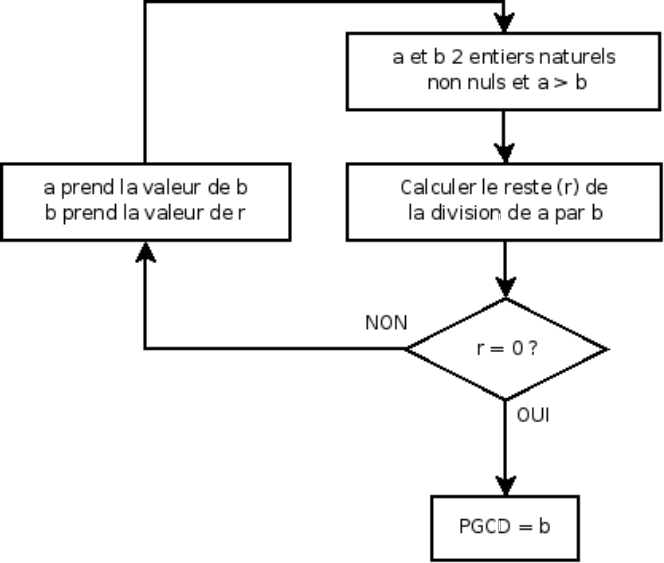
\includegraphics[width=.45\textwidth]{images/algo_euclide}
\end{center}
%\subsection{Recherche des nombres premiers -- Crible d'Ératosthène}
\subsection{Calcul de puissance}
\subsubsection{Algorithme naïf}

\begin{py}
\begin{python}
def exponentiation_naive(x,n):
    """
    Renvoie x* *n par la methode naive.
    Keyword arguments:
    Entrées : 
        x, flt : un nombre réel
        n, int : un nombre entier
    Sortie : 
        res,flt : resultat
    """
    res = 1
    while n>=1:
        res = res * x
        n=n-1
    return res
\end{python}
\end{py}

\subsubsection{Exponentiation rapide itérative}
\begin{py}
\begin{python}
def exponentiation_rapide_iteratif(x,n):
    """ 
    Renvoie x**n par la methode d'exponentiation rapide.
    Keyword arguments:
    Entrées : 
        x, flt : un nombre réel
        n, int : un nombre entier
    Sortie : 
        res,flt : resultat
    """
    if n==0 :
        return 1
    else :
        res = 1
        a = x
        while n>0:
            if n%2 == 1:
                res = res*a
            a=a*a
            n=int(n/2)
        return res
\end{python}
\end{py}


%\section{Calcul d'un polynôme}
%\subsection{Algorithme naïf}
%\subsection{Méthode de Horner}

\begin{thebibliography}{2}
\bibitem{pb}{Patrick Beynet, Cours d'informatique de CPGE, Lycée Rouvière de Toulon, UPSTI.}
\bibitem{ap}{Adrien Petri et Laurent Deschamps, Cours d'informatique de CPGE, Lycée Rouvière de Toulon.}
\bibitem{di}{Damien Iceta, Cours d'informatique de CPGE, Lycée Gustave Eiffel de Cachan, UPSTI.}
\bibitem{wack}{Benjamin WACK, Sylvain CONCHON, Judicaël COURANT, Marc DE FALCO, Gilles DOWEK, Jean-Christophe FILLIÂTRE, Stéphane GONNORD, 
Informatique pour tous en classes préparatoires aux grandes écoles, 
Éditions Eyrolles.}
\end{thebibliography}
\end{document}


 